%\documentclass{article}
\documentclass{colt2015} % Anonymized submission
\usepackage{hyperref}
\usepackage{url}
\usepackage{times}
\usepackage[algo2e]{algorithm2e}

%\usepackage{fullpage}
%\usepackage{amsmath,amsfonts,amsthm,amssymb}
\usepackage{bbm}
\usepackage{graphics, graphicx, xcolor}
\usepackage{enumitem}
\usepackage{verbatim}		% for misc commenting, etc.
\usepackage{stmaryrd}
\usepackage[mathscr]{euscript}

\newtheorem{thm}{Theorem}%[section]
\newtheorem{lem}[thm]{Lemma}
\newtheorem{prop}[thm]{Proposition}
\newtheorem{cor}[thm]{Corollary}
\newtheorem{conj}[thm]{Conjecture}
\newtheorem{obs}[thm]{Observation}
\newtheorem{defn}[thm]{Definition}
\newtheorem{alg}{Algorithm}
\newtheorem{ass}{Assumption}
\newtheorem{examp}{Example}
\newtheorem{property}{Property}
\setcounter{MaxMatrixCols}{20}

\newcommand{\corr}{\mbox{corr}}
\newcommand{\ones}[1]{\mathbbm{1}^{#1}}
\newcommand{\vA}{\mathbf{A}}
\newcommand{\va}{\mathbf{a}}
\newcommand{\vd}{\mathbf{d}} 
\newcommand{\vf}{\mathbf{f}}
\newcommand{\vF}{\mathbf{F}} 
\newcommand{\vI}{\mathbf{I}}  
\newcommand{\vh}{\mathbf{h}}
\newcommand{\vx}{\mathbf{x}}
\newcommand{\vb}{\mathbf{b}} 
\newcommand{\vu}{\mathbf{u}}   
\newcommand{\vl}{\mathbf{l}}
\newcommand{\vm}{\mathbf{m}}    
\newcommand{\vg}{\mathbf{g}}   
\newcommand{\vp}{\mathbf{p}}
\newcommand{\vq}{\mathbf{q}}
\newcommand{\vr}{\mathbf{r}}
\newcommand{\vs}{\mathbf{s}}
\newcommand{\vt}{\mathbf{t}}
\newcommand{\vv}{\mathbf{v}}
\newcommand{\vw}{\mathbf{w}}
\newcommand{\vz}{\mathbf{z}}
\newcommand{\valpha}{\vec{\alpha}}
\newcommand{\vbeta}{\vec{\beta}}
\newcommand{\vzero}{\mathbf{0}}
\newcommand{\vone}{\mathbf{1}}

\DeclareMathOperator{\id}{id}
\DeclareMathOperator{\tr}{tr}
\DeclareMathOperator*{\argmin}{arg\,min}
\DeclareMathOperator*{\argmax}{arg\,max}
\DeclareMathOperator{\sgn}{sgn}
\DeclareMathOperator{\Prtxt}{Pr}
\DeclareMathOperator{\var}{var}
\DeclareMathOperator{\poly}{poly}
\DeclareMathOperator{\polylog}{polylog}

\newcommand{\bd}[1]{\mathbf{#1}}  % for bolding symbols
\newcommand{\RR}{\mathbb{R}}      % Real numbers
\newcommand{\ZZ}{\mathbb{Z}}      % Integers
\newcommand{\NN}{\mathbb{N}}      % natural numbers
\newcommand{\RP}{\mathbb{RP}}      % real projective space
\newcommand{\Sp}{\mathbb{S}}
\newcommand{\HH}{\mathbb{H}}
\newcommand{\col}[1]{\left[\begin{matrix} #1 \end{matrix} \right]}
\newcommand{\comb}[2]{\binom{#1^2 + #2^2}{#1+#2}}
\newcommand{\vnorm}[1]{\left\lVert#1\right\rVert} % vector norm
\newcommand{\bfloor}[1]{\left\lfloor#1\right\rfloor} % floor function
\newcommand{\bceil}[1]{\left\lceil#1\right\rceil} % ceiling function
\newcommand{\ifn}{\mathbf{1}} % indicator function for sets
\newcommand{\EV}{\mathbb{E}} % expected value operator
\newcommand{\evp}[2]{\mathbb{E}_{#2} \left[#1\right]} % expected value operator
\newcommand{\abs}[1]{\left| #1 \right|}
\newcommand{\pr}[1]{\Prtxt \left(#1\right)}
\newcommand{\prp}[2]{\Prtxt_{#2} \left(#1\right)}
\newcommand{\ip}[2]{\left\langle #1, #2 \right\rangle}
\newcommand{\err}[1]{\mbox{err}\left(#1\right)}
\newcommand{\emperr}[2]{\widehat{\mbox{err}}_{#2} \left(#1\right)}

\newcommand{\zbr}{\textsc{ZBR}}
\newcommand{\wmv}{\textsc{WMV}}
\newcommand{\ns}{\textsc{NS}}
\newcommand{\hc}{\mathscr{HC}}
\newcommand*{\qedinp}{\hfill\ensuremath{\blacksquare}} %in-place qed theorem box; black box
\newcommand*{\qedinpw}{\hfill\ensuremath{\square}} % white box

\newcommand{\pderiv}[2]{\frac {\partial \left[ #1 \right]} {\partial #2}}
\newcommand{\expp}[1]{\exp \left(#1\right)}
\newcommand{\epshat}{\hat{\epsilon}}
\newcommand{\sighat}{\hat{\sigma}}
\newcommand{\gamhat}{\hat{\gamma}}
\newcommand{\cH}{\mathcal{H}}
\newcommand{\cX}{\mathcal{X}}
\newcommand{\cY}{\mathcal{Y}}
\newcommand{\cZ}{\mathcal{Z}}
\newcommand{\cG}{\mathcal{G}}
\newcommand{\cD}{\mathcal{D}}
\newcommand{\cU}{\mathcal{U}}
\newcommand{\cS}{\mathcal{S}}
\newcommand{\cL}{\mathcal{L}}
\newcommand{\cN}{\mathcal{N}}
\newcommand{\cM}{\mathcal{M}}
\newcommand{\cF}{\mathcal{F}}
\newcommand{\cW}{\mathcal{W}}
\newcommand{\cE}{\mathcal{E}}
\newcommand{\cO}{\mathcal{O}}
\newcommand{\ctO}[1]{\tilde{\mathcal{O}}\left(#1\right)}
\newcommand{\Ve}{V_\epsilon}
\newcommand{\pdis}[1]{P_{dis}\left(#1\right)}
\newcommand{\lrp}[1]{\left(#1\right)}
\newcommand{\lrb}[1]{\left[#1\right]}
\newcommand{\lrsetb}[1]{\left\{#1\right\}}

\newcommand{\authcmt}[2]{\textcolor{#1}{}}
\newcommand{\akshay}[1]{\authcmt{red}{[AB: #1]}}
\newcommand{\yoav}[1]{\authcmt{blue}{[YF: #1]}}



\makeatletter
\def\blfootnote{\xdef\@thefnmark{}\@footnotetext}
\makeatother


\begin{document}

\title[Minimax Classifier Aggregation]{Optimally Combining Classifiers Using Unlabeled Data}

  % \coltauthor{\Name{Author Name1} \Email{abc@sample.com}\and
  %  \Name{Author Name2} \Email{xyz@sample.com}\\
  %  \addr Address}
\coltauthor{\Name{Akshay Balsubramani} \Email{abalsubr@ucsd.edu}\\
\Name{Yoav Freund} \Email{yfreund@ucsd.edu}\\
\addr 9500 Gilman Drive, La Jolla, CA 92093}


\maketitle

\begin{abstract}

We develop a worst-case analysis of aggregation of classifier ensembles for binary classification. 
The task of predicting to minimize error is formulated as a game played 
over a given set of unlabeled data (a transductive setting), 
where prior label information is encoded as constraints on the game. 
The minimax solution of this game identifies cases where a
weighted combination of the classifiers can perform significantly
better than any single classifier.

\end{abstract}
\begin{keywords}
Ensemble aggregation, transductive, minimax
\end{keywords}


% Remember to thank grant.

\section{Introduction}
Suppose that we have a finite set, or ensemble, of binary classifiers
$\cH = \{ h_1,h_2,\ldots,h_p \}$, 
with each $h_i$ mapping data in some space $\cX$ to a binary prediction $\{-1,+1\}$. 
Examples $(x,y) \in \cX \times \{-1,+1\}$ 
are generated i.i.d. according to some fixed but unknown distribution 
$\cD$ -- write the expectation with respect to $\cD$ or one of its marginal distributions as $\evp{\cdot}{\cD}$.

Consider a statistical learning setting, 
in which we assume access to two types of i.i.d. data: a small set of training examples  
$S = \{(x'_1,y'_1),\ldots(x'_m,y'_m)\}$ drawn from $\cD$ and a much larger
set of unlabeled test examples $T = \{x_1,\ldots,x_n\}$ drawn i.i.d. 
according to the marginal distribution over $\cX$ induced by $\cD$. 
A typical use of the labeled set is to find an upper bound on the expected error rate for each of the classifiers. 
Specifically, we assume a set of lower bounds $\{b_i>0\}_{i=1}^p$ such
that the correlation $\corr(h) := \evp{y h (x)}{\cD}$ satisfies
$\corr(h) \geq b_i$.

If we ignore the test set, then the best we can do, in the worst case,
is use the classifier with the largest correlation (smallest error).
This corresponds to the common practice of {\em Empirical Risk
  Minimization} (ERM).  However, in many cases we can glean useful
information from the distribution of the test set that will allow us
to greatly improve over ERM.

We motivate this statement by contrasting two simple cases, A and B. 
In both cases there are $p=3$ classifiers and $n=3$ unlabeled test
examples. The correlation vector is $(1/3,1/3,1/3)$; equivalently,
the classifier error rates are $33\%$.  Based on that information the predictor
knows that each classifier makes two correct predictions and one
incorrect prediction.

So far, both cases are the same. The difference is in the relations
between different predictions on the same example.  In case A, each
example has two predictions that are the same, and a third that is
different.  In this case it is apparent that the majority vote
over the three classifiers has to be correct on all 3 examples,
i.e. we can reduce the error from $\frac{1}{3}$ to $0$. In case B, all
three predictions are equal for all examples. In other words, the
three classification rules are equal on the three examples. In this
case, there is no way to improve over the single rules.

These cases show that there is information in the unlabeled test
examples that can be used to reduce error. In this paper, we give a
complete characterization of the minimax predictions given the
correlation vector $\vb$ and the unlabeled test examples.

Our development does not consider the instance space $\cX$ directly, 
but instead models the knowledge of the $p$ ensemble predictions on $T$ 
with a $p \times n$ matrix that we denote by $\vF$. Our focus is on
how to use the matrix $\vF$ in conjunction with the correlation
vector $\vb$, to make the minimax optimal predictions on the test examples.  

The rest of the paper is organized as follows.  In
Section~\ref{sec:setup} we introduce some additional notation.  In
Section~\ref{sec:game1} we define the game between the predictor and
nature and solve it, characterizing the minimax strategies for both
sides by minimizing a convex objective we call the slack function. 
After linking the game to statistical learning in Section \ref{sec:uniform-convergence}, in
Section~\ref{sec:discthmpred} we give some interpretation of the slack
function and the minimax strategies. In Section~\ref{sec:alg} we
focus on computational issues in computing the minimax strategy.  After discussing relations to other work in
Section~\ref{sec:relwork}, we conclude in
Section~\ref{sec:openproblems}.

\section{Preliminaries}
\label{sec:setup}

The main tools we use in this paper are linear programming and uniform
convergence. We therefore use a combination of matrix notation and
probabilistic notation. The probabilistic notation was given in
the introduction. The algorithm is described in a deterministic
context where some inequalities are assumed to hold; probabilistic
arguments are used to show that these assumptions are correct with high
probability.

The ensemble's predictions on the unlabeled data are denoted by $\vF$:
\begin{equation}
\vF = 
 \begin{pmatrix}
   h_1(x_1) & h_1(x_2) & \cdots & h_1 (x_n) \\
   h_2(x_1) &  h_2(x_2) & \cdots & h_2 (x_n) \\
   \vdots   & \vdots    & \ddots &  \vdots  \\
   h_p(x_1)  &  h_p (x_2)  & \cdots &  h_p (x_n)
 \end{pmatrix}
 \in [-1, +1]^{p \times n}
\end{equation}

Note that we allow $\vF$, as well as other variables defined below, to
take any value in the range $[-1,+1]$ rather than just the two
endpoints. This relaxation does not change the analysis, because intermediate
values can be interpreted as the expected value of randomized
predictions.  For example, a value of $\frac{1}{2}$ indicates $\{+1\;
\text{w.p.}\; \frac{3}{4} $, $-1\; \text{w.p.}\; \frac{1}{4} \}$. This
interpretation extends to our definition of the empirical correlation
on the test set,
$\hat{\corr}(h) = \frac{1}{n} \sum_{i=1}^n h(x_i)y_i$.~\footnote{We are slightly abusing the
  term ``correlation'' here. Strictly speaking this is the expected
  value of the product without subtracting means and dividing by the
  product of the standard deviations. We prefer this to
  inventing a new term.}

We use vector notation for the rows and columns of $\vF$: 
$\vh_i = (h_i(x_1), h_i(x_2), \cdots, h_i (x_n))^\top$ and \\$\vx_j =
(h_1(x_j), h_2(x_j), \cdots, h_p (x_j))^\top$.

The \textbf{true labels} on the test data $T$ are represented by $\vz
= (z_1; \dots; z_n) \in [-1,1]^n$. The labels $\vz$ are hidden from the predictor, 
but we assume the predictor has knowledge of a {\bf correlation vector}
$\vb \geq \vzero^n$ such that $ \frac{1}{n} \sum_j h_i (x_j) z_j \geq b_i$, 
i.e. $ \frac{1}{n} \vF \vz \geq \vb$. 

We establish the following notation: $[a]_{+} = \max (0, a)$ and $[a]_{-} = [-a]_{+}$,  
$[n] = \{ 1,2,\dots,n \}$, $\vone^n = (1; 1; \dots; 1) \in \RR^n$, and $\vzero^n$
similarly.  Also, write $I_n$ as the $n \times n$ identity matrix.
All vector inequalities are componentwise. 

The probability simplex in $d$ dimensions is denoted by $\Delta^d = \{ x \geq \vzero^d : \sum_{i=1}^d x_i = 1 \}$.

%----------------------------------------------------------------------------------------------------------------------------------------------------------------------------------------------------------------------------------


\section{The Transductive Binary Classification Game}
\label{sec:game1}

We now describe our prediction problem, and formulate it as a
two-player zero-sum game between a predictor and nature.

In this game, the predictor is the first player, 
who plays $\vg = (g_1; g_2; \dots; g_n)$, 
a randomized label $g_i \in [-1,1]$ for each example $\{\vx_i\}_{i=1}^{n}$. 
Nature then plays adversarially, setting the labels $\vz \in [-1,1]^n$ 
under ensemble error constraints defined by $\vb$. 
The predictor's goal is to minimize (and Nature's to maximize) 
the \emph{worst-case expected classification error on the test data} 
(w.r.t. the randomized labelings $\vz$ and $\vg$): 
$\frac{1}{2} \lrp{1 - \frac{1}{n} \vz^\top \vg }$. 
This is equivalently viewed as maximizing worst-case correlation $\frac{1}{n} \vz^\top \vg $. 

To summarize concretely, we study the following game:
\begin{align}
\label{game1eq}
\displaystyle 
V\doteq\max_{\vg \in [-1,1]^n} \; \min_{\substack{ \vz \in [-1,1]^n , \\ \frac{1}{n} \vF \vz \geq \vb }} \;\; \frac{1}{n} \vz^\top \vg
\end{align}

It is important to note that we are only modeling ``test-time''
prediction, and represent the information gleaned from the labeled data
by the parameter $\vb$. Inferring the vector $\vb$ from training data
is a standard application of Occam's Razor, which we provide in
Section~\ref{sec:uniform-convergence}.

The minimax theorem (e.g. \cite{CBL06}, Theorem 7.1) applies to the game \eqref{game1eq}, 
since the constraint sets are convex and compact and the payoff linear. 
Therefore, it has a minimax equilibrium and associated optimal 
strategies $\vg^*, \vz^*$ for the two sides of the game, i.e. 
$\min_{\vz}\; \frac{1}{n} \vz^\top \vg^* = V = \max_{\vg} \frac{1}{n} \vz^{*^\top} \vg$ .
%\begin{align*}
%\min_{\substack{ \vz \in [-1,1]^n , \\ \frac{1}{n} \vF \vz \geq \vb }}\; \frac{1}{n} \vz^\top \vg^* 
%= V = \max_{\vg \in [-1,1]^n} \frac{1}{n} \vz^{*^\top} \vg
%\end{align*}

As we will show, both optimal strategies are simple functions of a
particular weighting over the $p$ hypotheses -- a nonnegative $p$-vector. 
Define this weighting as follows.
\begin{defn}[\textbf{Slack Function}]
Let $\sigma \geq 0^p$ be a weight vector over $\cH$ (not necessarily a distribution).
The vector of \textbf{ensemble predictions} is
$\vF^\top \sigma = (\vx_1^\top \sigma, \dots, \vx_n^\top \sigma)$, 
whose elements' magnitudes are the \textbf{margins}. 
The \textbf{prediction slack function} is
\begin{align}
\label{eqn:slack}
\gamma (\sigma, \vb) \doteq \gamma (\sigma) \doteq \frac{1}{n} \sum_{j=1}^n \left[ \abs{\vx_{j}^\top \sigma} - 1 \right]_{+} - \vb^\top \sigma
\end{align}
\end{defn}
\begin{defn}[\textbf{Optimal Weight Vector}]
The \textbf{optimal weight vector} $\sigma^*$ is any minimizer of the slack function: 
$\displaystyle \sigma^* \in \argmin_{\sigma \geq 0^p} \left[ \gamma (\sigma) \right]$.
\end{defn}

Our main result uses these to describe the minimax equilibrium of the game \eqref{game1eq}.
\begin{thm}[Solution of the Game]
\label{thm:gamesolngen}
The minimax value of the game \eqref{game1eq} is 
$V = - \gamma (\sigma^*)$. 
The minimax optimal strategies are defined as follows:
for all $i \in [n]$,
\begin{align}
g_i^* \doteq g_i (\sigma^*) = \begin{cases} x_{i}^\top \sigma^* & \abs{x_{i}^\top \sigma^*} < 1 \\ 
\sgn(x_{i}^\top \sigma^*) & otherwise \end{cases}
\quad \quad \text{and} \quad \quad
z_i^* = 
\begin{cases} 
0 & \abs{x_{i}^\top \sigma^*} < 1 \\ 
\sgn(x_{i}^\top \sigma^*) & \abs{x_{i}^\top \sigma^*} > 1 
\end{cases}
\label{eqn:opt-strats}
\end{align}
\end{thm}

\begin{figure}
\centering
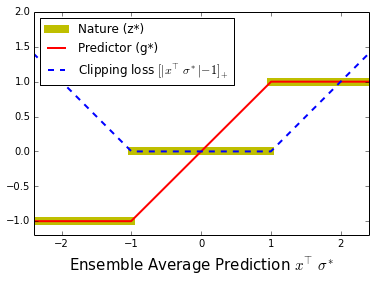
\includegraphics[width=0.55\textwidth]{figs/optstrats.png}
\caption{
\label{fig:optstrats}
The optimal strategies and slack function as a function of the ensemble prediction $x^\top \sigma^*$.}
\end{figure}

The proof of this theorem involves linear program analysis.
The minimax value of the game (proved in Lemma \ref{lem:valgame1}) and 
the optimal strategy for the predictor $\vg^*$ (Lemma~\ref{lem:game1gopt}) 
are our main objects of study and are completely characterized, 
and the theorem's partial description of $\vz^*$ (proved in Lemma \ref{lem:game1zopt}) 
will suffice for our purposes. 
\footnote{For completeness, Corollary \ref{cor:zoptfullpred} in the appendices 
specifies $z_i^*$ when $\abs{x_{i}^\top \sigma^*} = 1$.}

Theorem \ref{thm:gamesolngen} illuminates the importance of the optimal weighting $\sigma^*$ over hypotheses. 
This weighting $\sigma^* \in \argmin_{\sigma \geq 0^p} \gamma (\sigma)$ is the solution 
to a convex optimization problem (Lemma \ref{lem:helperthreshcvx}), 
and therefore we can efficiently compute it and $\vg^*$ to any desired accuracy. 
The ensemble prediction (w.r.t. this weighting) on the test set is $\vF^\top \sigma^*$, 
which is the only dependence of the optimal solution on $\vF$.
More specifically, the minimax optimal prediction/label \eqref{eqn:opt-strats} on any test set example $\vx_j$ 
can be expressed as a function of the ensemble prediction $\vx_j^\top \sigma^*$.
These functions are depicted in Figure \ref{fig:optstrats}. 



%------------------------------------------------------------------------------------------------------------------------------------------------------------------------------------------
\section{Bounding the Correlation Vector}
\label{sec:uniform-convergence}

In the analysis presented above we assumed that a correlation vector
$\vb$ is given and that it is guaranteed to be a lower bound  on the
true correlations on the test set. In this section we analyze how
$\vb$ can be calculated from a labeled training set.

The algorithm that we use is the natural one: we compute the empirical
correlation for the $p$ classifiers and add a uniform penalty term to guarantee
that the $\vb$ is a lower bound on the correlation of the test data.

For each classifier, we have three quantities to consider:
\begin{itemize}
\item The true correlation: $\corr(h) = \evp{y h(x)}{\cD}$
\item The correlation on the training set: $\widehat{\corr}_{\mbox{trn}}(h) =
  \frac{1}{m} \sum_{i=1}^m h(x'_i)y'_i$
\item The correlation on the test set: $\widehat{\corr}_{\mbox{tst}}(h) =
  \frac{1}{n} \sum_{i=1}^n h(x_i)y_i$
\end{itemize}
Using Chernoff bounds, we can bound the probability that each of the empirical
correlations is $\epsilon$ far from the true correlation. For each
individual classifier we have the inequalities 
\begin{eqnarray*}
\pr{\widehat{\corr}_{\mbox{trn}} > \corr(h)+\epsilon_{\mbox{trn}}} \leq e^{-2m \epsilon^2} \\
\pr{\widehat{\corr}_{\mbox{tst}} < \corr(h)-\epsilon_{\mbox{tst}}} \leq e^{-2n \epsilon^2} 
\end{eqnarray*}

Let $\delta$ denote the probability we allow for failure. If we set 
$\epsilon_{\mbox{trn}}=\sqrt{(\ln(p/\delta))/2m}$ and
$\epsilon_{\mbox{tst}}=\sqrt{(\ln(p/\delta))/2n}$, we are guaranteed that {\em
  all} of the inequalities hold concurrently with probability at
least $1-\delta$.

We thus set the correlation bound to:
\[
b_i=\widehat{\corr}(h_i)-\sqrt{(\ln(p/\delta))/2m}-\sqrt{(\ln(p/\delta))/2n}
\]
and have that $\vb$ is a good correlation vector with probability $1-\delta$.

%------------------------------------------------------------------------------------------------------------------------------------------------------------------------------------------


\section{Discussion}
\label{sec:discthmpred}

Given $\sigma$, we partition the examples $\vx$ into three subsets, depending on the value of the ensemble prediction: 
the {\bf hedged set} $ H (\sigma) := \left\{ \vx :  |\vx^\top \sigma|<1 \right\} $, 
the {\bf clipped set} $C (\sigma) := \left\{ \vx :  |\vx^\top \sigma|>1 \right\} $, 
and the {\bf borderline set} $B (\sigma) \doteq \left\{ \vx :  |\vx^\top \sigma|=1 \right\} $.
Using these sets, we now give some intuition regarding the optimal
choice of $\vg$ and $\vz$ given in~(\ref{eqn:opt-strats}), for some fixed $\sigma$.

Consider first examples $\vx$ in $H(\sigma)$. The optimal strategy for the predictor is
to predict with the ensemble average $\vx^\top \sigma$, which is
a number between $-1$ and $+1$. Making such an intermediate prediction
might seem to be a type of calibration, but this view is misleading. The
optimal strategy for the adversary in this case is to set $\vz_i=0$, 
equivalent to predicting $\pm 1$ with probability $1/2$ each. 
The reason that the learner hedges is because if $g < \vx^\top \sigma$, 
the adversary would respond with $z=1$
and with $z=-1$ if $g > \vx^\top \sigma$. 
In either case, the loss of the predictor would increase. 
In other words, our ultimate rationale for hedging is not calibration, 
but rather ``defensive forecasting'' in the spirit of \cite{VTS05}.

Next we consider the clipped set $\vx \in C(\sigma)$. In this case, Nature's optimal strategy
is to predict deterministically, and so the learner matches Nature. It
is interesting to note that with all else held equal, increasing the margin 
$\abs{\vx_j^\top \sigma}$ beyond 1 is sub-optimal for the learner. 
Qualitatively, the reason is that while $\vx_j^\top \sigma$
continues to increase, the prediction for the learner is clipped, 
and so the value for the learner does not increase with the ensemble prediction.

\subsection{Subgradient Conditions}
For another perspective on the result of Theorem~\ref{thm:gamesolngen}, 
consider the subdifferential set of the slack function $\gamma$ at an arbitrary weighting $\sigma$:
\begin{align}
\label{subdiffgammasig}
\partial \gamma (\sigma) 
= \left\{ \frac{1}{n} \lrp{ \sum_{\vx_j \in C(\sigma)} \vx_j \sgn(\vx_j^\top \sigma) 
+ \sum_{\vx_j \in B(\sigma)} c_j \vx_j \sgn(\vx_j^\top \sigma) } - \vb
, \quad \forall c_j \in [0,1]  \right\}
\end{align}
Note that the hedged set plays no role in the gradient.
Since the slack function $\gamma(\cdot)$ is convex (Lemma \ref{lem:helperthreshcvx}), 
the sub-differential set \eqref{subdiffgammasig} at any $\sigma^*$ contains $\vec{0}$, 
i.e.,
\begin{align}
\label{gammasgexact}
\exists c_j \in [0,1] \qquad s.t. \qquad 
n \vb - \sum_{j : x_{j}^\top \sigma^* > 1} x_{j} + \sum_{j : x_{j}^\top \sigma^* < -1} x_{j} 
&= \sum_{j : \abs{x_{j}^\top \sigma^*} = 1} c_j x_{j} \sgn(x_{j}^\top \sigma^*)
\end{align}
The geometric interpretation of this equation is given in Figure~\ref{fig:optsigma}. 
The optimal weighting $\sigma^*$ partitions the examples into five sets: 
hedged, positive borderline and positive clipped, and negative borderline and negative clipped. 
Taking the difference between the sum of the positive clipped and the sum of the negative
clipped examples gives a vector that is approximately $\vb$. 
By adding a weighted sum of the borderline examples, $\vb$ can be obtained exactly.

\begin{figure}
\label{fig:optsigma}
\centering
\includegraphics[width=0.6\textwidth]{figs/Opt-Sigma.pdf}
\caption{\small An illustration of the optimal $\sigma^* \geq 0^p$. 
The vector $n \vb$ is the difference between the sums of two categories of clipped examples: 
those with high ensemble prediction ($x^\top \sigma^* > 1$) and low prediction ($< -1$).
The effect of $\{ x : \abs{x^\top \sigma^*} = 1\}$ is neglected for simplicity. 
}
\end{figure}

\iffalse 
\yoav{I don't think this duality, while true,  gives much insight}

A significant observation to make as we begin 
is that predictions of the form $\vg (\sigma)$ 
are closely related to dual optima and the slack function. 
Indeed, by definition of $\vg (\sigma)$, the slack function value 
$ - \gamma (\sigma) = b^\top \sigma - \frac{1}{n} \vnorm{\vF^\top \sigma - \vg (\sigma)}_1 
\leq \max_{\sigma' \geq 0^p} \left[ b^\top \sigma' - \frac{1}{n} \vnorm{\vF^\top \sigma' - \vg (\sigma)}_1 \right]$, 
which is simply the dual problem (Lemma \ref{lem:gamegeng}) of the worst-case correlation suffered by $\vg (\sigma)$: 
$\displaystyle \quad \min_{\substack{ \vz \in [-1,1]^n , \\ \frac{1}{n} \vF \vz \geq \vb }} \;\frac{1}{n} \vz^\top [\vg (\sigma)]$. 
We now state this formally.
\begin{obs}
\label{obs:slacksubopt}
For any weight vector $\sigma \geq 0^p$, 
the worst-case correlation after playing $\vg (\sigma)$ is bounded by 
$\displaystyle \quad \min_{\substack{ \vz \in [-1,1]^n , \\ \frac{1}{n} \vF \vz \geq \vb }} \;\frac{1}{n} \vz^\top [\vg (\sigma)] 
\geq - \gamma (\sigma) $\;.
\end{obs}
%--------------------------------------------------------------------------------------------------------------------------
\fi

\subsection{Better than ERM Without Clipping}
We now make some simple observations about the minimax solution.

First, note that no $\sigma$ such that $\vnorm{\sigma}_1 < 1$ can be optimal, 
because in such a case $-\gamma(\sigma) > -\gamma \lrp{\frac{\sigma}{\vnorm{\sigma}_1}}$; 
therefore, $\vnorm{\sigma^*}_1 \geq 1$.

Consider next a situation where we do not know the matrix $\vF$. 
Then $\|\sigma^*\|_1=1$. This can be shown by proving the contra-positive; 
assume the negation $\|\sigma^*\|_1 > 1$. Then there exists a 
vector $x \in [-1,+1]^p$ such that $x^\top \sigma^* = \|\sigma^*\|_1 > 1$. 
If each of the columns of $\vF$ is equal to $x$, 
then $\sigma^*$ cannot be optimal since 
$-\gamma \lrp{\frac{\sigma^*}{a}} > -\gamma(\sigma^*)$. 

In other words, if we want to protect ourselves against the worst case $\vF$, then
we have to set $\|\sigma\|_1=1$ so as to ensure that $C(\sigma)$ is empty. 
In this case, the slack function simplifies to $\gamma (\sigma) = - \vb^\top \sigma$, 
over the probability simplex. 
Minimizing this is achieved by setting $\sigma_i$ to be $1$ at $\displaystyle \argmax_{i \in [p]} b_i$ and zero
elsewhere. As might be expected, in the case that $\vF$ is unknown, the
optimal strategy is to use the classifier with the minimal error guarantee. 

This is because $C(\sigma^*)$ is empty, 
and the set of all $\sigma$ such that this is true is of wider interest. 
We name it the \emph{Zero Box Region}: $\zbr = \left\{ \sigma : C(\sigma) = \emptyset \right\}$.
Another clean characterization of the $\zbr$ can be made by using a 
duality argument similar to that used to prove Theorem \ref{thm:gamesolngen}. 

\begin{thm}
\label{thm:zbrunconstr}
The best weighting in $\zbr$ satisfies 
$\displaystyle \max_{\substack{ \abs{\vF^\top \sigma} \leq \mathbf{1}^n , \\ \sigma \geq 0^p }} \; \vb^\top \sigma 
= \max_{\vg \in [-1,1]^n} \;\min_{\frac{1}{n} \vF \vz \geq \vb } \;\; \frac{1}{n} \vz^\top \vg  $\;. 
In particular, the optimal $\sigma^* \in \zbr$ if and only if 
the hypercube constraint $\vz \in [-1,1]^{n}$ is superfluous, i.e. when 
$\displaystyle V = \min_{ \frac{1}{n} \vF \vz \geq \vb } \;\max_{\vg \in [-1,1]^n} \;\; \frac{1}{n} \vz^\top \vg $\;.
\end{thm}
The $\zbr$ is where the optimal strategy is always to hedge 
and never to incorporate any clipping. 
\iffalse
\yoav{I don't understand this sentence.}
So Theorem \ref{thm:zbrunconstr} states that the 
hypercube constraint $\vz \in [-1,1]^n$ exactly corresponds 
to the presence of clipping in $\vg$. 
\fi
Consider a situation in which the solution is in $\zbr$, $\sigma^*=\ones{p}$, 
and all of the predictions are binary: $\vF \in \{-1,+1\}^{p \times n}$.
This is an ideal case for our method; instead of the baseline value $\max_i b_i$
obtained when $\vF$ is unknown, we get a superior value of $\sum_i b_i$. 

In fact, we referred to such a case in the introduction, 
and we will present a formal version here. 
Take $p$ to be odd and suppose that $n=p$. 
Then set $\vF$ to be a matrix where each row (classifier) and each column (example)
contains $(p+1)/2$ entries equal to $+1$ and $(p-1)/2$ entries equal to $-1$.
\footnote{For instance, by setting $F_{ij} = 2 * \ifn((i+j) \text{ is even}) - 1$.} 
Finally choose an arbitrary subset of the columns (to have true label $-1$), 
and invert all their entries. 

In this setup, all classifiers (rows) have the same error: $\vb= \frac{1}{p} \ones{p}$. 
The optimal weight vector in this case is $\sigma^*=\ones{p}$, 
the solution is in $\zbr$ because $\abs{x^\top \sigma^*} = 1 \;\forall x$, and the minimax value is $V=1$, 
which corresponds to zero error. 
Any single rule has an error of $\frac{1}{2} - \frac{1}{p}$, 
so using $\vF$ with $p$ classifiers has led to a $p$-fold improvement over random guessing!

Of course, this particular case is extremal in some ways; in order to be in $\zbr$, 
there must be many cancellations in $\vF^\top \sigma^*$. 
This echoes the common belief that, when combining an ensemble of classifiers, 
we want the classifiers to be ``diverse" (e.g. \cite{K03}). 
The above example in fact has the maximal average disagreement between pairs of classifiers for a fixed $p$. 
Similar results hold if $\vF$ is constructed using independent random draws.


Another consequence of our formulation 
is that predictions of the form $\vg (\sigma)$ 
are closely related to dual optima and the slack function. 
Indeed, by definition of $\vg (\sigma)$, the slack function value 
$ - \gamma (\sigma) = b^\top \sigma - \frac{1}{n} \vnorm{\vF^\top \sigma - \vg (\sigma)}_1 
\leq \max_{\sigma' \geq 0^p} \left[ b^\top \sigma' - \frac{1}{n} \vnorm{\vF^\top \sigma' - \vg (\sigma)}_1 \right]$, 
which is simply the dual problem (Lemma \ref{lem:gamegeng}) of the worst-case correlation suffered by $\vg (\sigma)$: 
$\displaystyle \quad \min_{\substack{ \vz \in [-1,1]^n , \\ \frac{1}{n} \vF \vz \geq \vb }} \;\frac{1}{n} \vz^\top [\vg (\sigma)]$. 
We now state this formally.

\begin{obs}
\label{obs:slacksubopt}
For any weight vector $\sigma \geq 0^p$, 
the worst-case correlation after playing $\vg (\sigma)$ is bounded by 
$$ \quad \min_{\substack{ \vz \in [-1,1]^n , \\ \frac{1}{n} \vF \vz \geq \vb }} \;\frac{1}{n} \vz^\top [\vg (\sigma)] 
\geq - \gamma (\sigma) $$
\end{obs}




\subsection{Independent Label Noise}

An interesting variation on the game is to limit the adversary to 
$z_i \in [-\alpha_i,\alpha_i]^n$ for some $\vec{\alpha} = (\alpha_1 ; \dots ; \alpha_n) \in [0,1)^n$. 
This corresponds to assuming a level $1 - \alpha_i$ of independent label noise on example $i$: 
the adversary is not allowed to set the label deterministically, 
but is forced to flip example $i$'s label independently 
with probability $\frac{1}{2}(1 - \alpha_i)$. 

Solving the game in this case gives the result (proof in appendices) 
that if we know some of the ensemble's errors to be through random noise, 
then we can find a weight vector $\sigma$ that would give us better performance than 
without such information. 
\begin{prop}[Independent Label Noise]
\label{prop:labnoise}
\begin{align*}
\max_{\vg \in [-1,1]^n} \;\;\min_{\substack{ - \valpha \leq \vz \leq \valpha , \\ 
\frac{1}{n} \vF \vz \geq \vb }} \;\; \frac{1}{n} \vz{^\top} \vg 
= \max_{\sigma \geq 0^p } \;\;\vb^\top \sigma - \frac{1}{n} \sum_{j=1}^n \alpha_j \left[ \abs{x_{j}^\top \sigma} - 1 \right]_{+}
> \max_{\sigma \geq 0^p } \;[- \gamma (\sigma)]
= V 
\end{align*}
\end{prop}
Our prediction tends to clip -- predict with the majority vote -- more on examples with more known random noise, 
because it gains in minimax correlation by doing so. 
This mimics the Bayes-optimal classifier, which is always a majority vote. 

Indeed, this statement's generalization to the asymmetric-noise case 
can be understood with precisely the same intuition. 
The sign of the majority vote affects the clipping penalty in the same way:
\begin{prop}[Asymmetric Label Noise] 
For some $\vl, \vu \geq \vzero^n$,
\begin{align*}
\max_{\vg \in [-1,1]^n} \;\;\min_{\substack{ -\vl \leq \vz \leq \vu , \\ 
\frac{1}{n} \vF \vz \geq \vb }} \;\; \frac{1}{n} \vz{^\top} \vg 
= \max_{\sigma \geq 0^p } \;\;\vb^\top \sigma - \frac{1}{n} \sum_{j=1}^n \lrp{ u_j \left[ x_{j}^\top \sigma - 1 \right]_{+} + l_j \left[ - x_{j}^\top \sigma - 1 \right]_{+} }
> V 
\end{align*}
\end{prop}







\iffalse
\akshay{If there's space: Point out that feasibility conditions make this a statement about 
\emph{where we know the errors are coming from}, countering the naive objection that ``adding noise should not ever increase performance." }

As a further aid to intuition, 
consider the following scenario. 
\akshay{I'll rewrite this example.}
\begin{example}
\label{ex:combavgvote}
Suppose the data are divided into two subsets, 
with a fraction $1-\alpha$ being in $\cX_1$ and $\alpha$ in $\cX_2$ for some $\alpha \in [0,1]$. 
Also suppose all $p$ hypotheses predict with zero errors on $\cX_1$, 
and each makes errors on a fraction $\epsilon$ of $\cX_2$ chosen uniformly at random. 
Then w.h.p. we have that the examples in $\cX_1$ all have margin $1$, 
those in $\cX_2$ have margin $1 - 2 \epsilon$, 
and $\vb$ is $(1 - 2 \epsilon \alpha) \vone^p$.
\end{example}
\akshay{
In Example \ref{ex:combavgvote}, the ZBR consists of weightings $\sighat$ with $\vnorm{\sighat}_1 \leq 1$, 
since the examples in $\cX_1$ have margin $1$ under all distributions. 
However, the optimal strategy is $\sigma^* = \frac{1}{p (1 - 2 \epsilon)} \vone^p$, 
an unweighted majority vote with zero error: $V = -\gamma(\sigma^*) = 1$. 
Choosing $\vnorm{\sigma^*}_1 > 1$ forces the examples in $\cX_1$ to have margin $> 1$, 
but the hypotheses' errors are low enough to make this introduction of voting effects worthwhile.
}

At the other end of the spectrum from the $\zbr$ is the scenario 
in which as much as possible, every prediction is clipped or borderline. 
For the optimal $\vg^* = \vg (\sigma^*)$ to be such a strategy, 
it must be of the form $\vg_{\wmv} (\sigma^*) = \sgn(F^\top \sigma^*)$, 
which is familiar as a \emph{weighted majority vote} ($\wmv$). 

There is a necessary subtlety in our definitions: the examples such that 
the ensemble prediction $x^\top \sigma^* = 0$ have no clear majority prediction, 
and therefore cannot be clipped or borderline in an optimal strategy - 
they must be hedged perfectly randomly. 
The set of such examples warrants special mention because of its role in the literature 
(see Section \ref{sec:relwork} for details). 

\begin{defn}[Hard Core w.r.t. $\sigma$]
The \emph{hard core} with respect to any weighting $\sigma \geq 0^p$ is the set 
\begin{align*}
\hc (\sigma) = \lrsetb{ x : x^\top \sigma = 0 }
\end{align*}
\end{defn}
In our setup, any optimal strategy must be of the form $\vg (\sigma)$ for some $\sigma$. 
So if $\wmv(\sigma)$ is optimal, it must predict with $0$ on $\hc (\sigma)$, 
therefore making errors on at least $\frac{1}{2} \prp{\hc (\sigma)}{}$. 
So the hard core limits the performance of the optimal strategy. 

Other than this limitation, however, we might expect that when the optimal strategy is a $\wmv$ 
that predicts as decisively as possible on all examples, it would perform quite well. 
Indeed, this can be formally shown (proof in appendices).
\begin{thm}
\label{thm:wmvoptcond}
Suppose a weighted majority vote using a weighting $\sigma \geq 0^p$ 
is the optimal strategy $\vg^* = \vg_{\wmv} (\sigma)$ for the game \eqref{game1eq}.
Then the expected classification error $\epsilon_{\wmv} (\sigma) = \frac{1}{2} (1-V)$ is bounded by: 
\begin{align*}
\frac{1}{2} \prp{\hc (\sigma)}{} 
\leq \epsilon_{\wmv} (\sigma)
\leq \frac{1}{2} \lrp{ \prp{\hc (\sigma)}{} + \prp{ \abs{x_j^\top \sigma} = \min_{x \notin \hc(\sigma)} \abs{x^\top \sigma} }{j}}
\end{align*}
\end{thm}


This shows that a WMV is minimax optimal only if it essentially matches the true labels exactly where it can, 
as in Example \ref{ex:combavgvote}. 
But in other cases, it is better for there to be some examples $i$ on which 
the predictor hedges ($\abs{g_i} < 1$), as indicated by $\vg^*$. 

\akshay{I can't prove an analogous result to Thm. \ref{thm:zbrunconstr}, 
But I think we need an example here where it is better to hedge at all. \\ \\
On another note, I have an error bound on an arbitrary WMV as well in terms of its margins - 
but that might exceed our scope here.}

\fi



%------------------------------------------------------------------------------------------------------------------------------------------------------------------------------------------
%------------------------------------------------------------------------------------------------------------------------------------------------------------------------------------------




\section{Computational Issues}
\label{sec:alg}
Theorem \ref{thm:gamesolngen} makes clear that our ability to produce $\vg^*$ 
is dependent on our ability to find the optimal weighting $\sigma^*$, 
i.e. to minimize the slack function $\gamma (\sigma)$ over $\sigma \geq 0^p$. 
We discuss two extreme approaches to performing this minimization.

The most straightforward approach is to treat the problem as a linear
programming problem and use an LP solver. The main problem with this
approach is that it requires storing all of the examples in memory. As
unlabeled examples are typically much more plentiful than labeled
examples, this approach could be infeasible without further modification.

A different approach that exploits the structure of the equilibrium uses stochastic gradient descent. The fact
that the slack function is convex guarantees that this approach will converge to the global minimum. 
The convergence rate might be suboptimal, particularly near the intersections of hyperplanes 
in the piecewise-linear slack function surface. But the fact that SGD is an constant-memory algorithm is very attractive. 
In fact, the entire arsenal of stochastic convex optimization comes into play theoretically and practically 
-- the slack function is a sum of i.i.d. random variables. 
As such, it has a natural limiting object $\evp{\left[ \abs{x^\top \sigma} - 1 \right]_{+}}{x \sim \cD} - b^\top \sigma$ 
amenable to standard optimization techniques. 




\iffalse

\subsection{Algorithm Overview}
We first define some statistical learning notation quantifying the parameters of the problem. 

We define the \emph{limiting slack function} as 
$\gamma_\infty (\sigma) = \evp{\left[ \abs{x^\top \sigma} - 1 \right]_{+}}{x \sim \cD} - b^\top \sigma$, 
and the associated \emph{limiting optimal prediction/value} as $\sigma_{\infty}^* = \argmin_{\sigma \geq 0^p} \gamma_\infty (\sigma)$ 
and $V_{\infty} = - \gamma_\infty (\sigma_{\infty}^*)$. 
Our algorithm processes examples incrementally to approximately minimize $\gamma_\infty$ 
by forming unbiased estimates of the limiting slack function: 
$\gamma^m (\sigma) = \frac{1}{m} \sum_{j=1}^m \left[ \abs{x_{j}^\top \sigma} - 1 \right]_{+} - b^\top \sigma$ 
for i.i.d. data $x_1, \dots, x_m \in \RR^d$. 

The algorithm proceeds in epochs $t = 1, 2, \dots$. 
During epoch $t$, incoming unlabeled examples are processed one at a time. 
The algorithm selectively stores only some informative examples in a set $S_t$, 
and merely keeps aggregated statistics 
about the rest, in the form of a count $q_t$ and a vector $\mu_t \in \RR^p$. 
This goes on until $\abs{S_t} = k$, 
at which point the algorithm stops processing data for epoch $t$, 
having drawn $\abs{S_t} + q_t$ examples that epoch. 

The decision of whether to sample is made by tracking  
a small region $C_t \subset \RR_+^p$ of ``good" weightings; 
by construction, this always contains $\sigma_{\infty}^*$ and defines the scope of our attention. 
When $x_t$ is put in the same category (hedged, positive/negative clipped/borderline) 
by all weightings in $C_{t-1}$, 
its contribution to the gradient is effectively fixed for the optimization. 
So in this case, $x_t$ can be exactly accounted for by adding it to the sum $\mu_t$, 
and it is safe to deem $x_t$ non-informative thereafter. 
In this manner, the $k$ examples $S_t$ are selected 
such that they -- along with $\mu_t, q_t$ -- 
exactly describe $\gamma^{\abs{S_t} + q_t} (\sigma)$ within $C_{t-1}$.


To discuss this with more rigor, 
we introduce a form of the slack function that is explicitly written only in terms of informative examples. 
\begin{defn}
\label{def:approxslack}[\textbf{Shorthand Slack Function}]
For a set of examples $S$, define the \emph{shorthand slack function}
\begin{align*}
\gamhat (\sigma, S, \mu, q) 
&= \frac{1}{|S| + q} 
\lrp{ \sum_{x \in S} \left[ \abs{x^\top \sigma} - 1 \right]_{+} } 
+ \lrp{\frac{\mu}{|S| + q} - b}^\top \sigma - \frac{q}{|S| + q} 
\end{align*}
and write $\gamhat_t (\sigma) := \gamhat (\sigma, S_t, \mu_t, q_t)$.
\end{defn}
\begin{lem}
\label{lem:compressslack}
For any $\sigma \in C_{t-1}$, $\gamhat_t (\sigma) = \gamma^{|S_t| + q_t} (\sigma)$.
\end{lem}

Lemma \ref{lem:compressslack} tells us that we can simulate an SGD minibatch update 
of \emph{effective batch size} $|S_t| + q_t \geq k$ on epoch $t$ with storage for just $\cO(k)$ examples. 
Accordingly, our algorithm each epoch runs the subroutine \texttt{GDUpdate}, 
which performs a minibatch update using the shorthand slack function. 
%Since $\gamma^{|S_t| + q_t} (\sigma)$ and its gradient are unbiased estimators of 
%$\gamma_{\infty} (\sigma)$ and its gradient, 
So just as mini-batch SGD produces a $\sigma_t$ that converges to $\sigma_{\infty}^*$, 
ours does as well. 
In particular, we will find a bound on this convergence useful. 
(We do not attempt to optimize for constants in what follows.)
\begin{prop}[\cite{DGBSX12}]
\label{prop:sgdconvrate}
For some finite $C > 0$, w.p. $\geq 1-\delta$, for all $t$, 
$$ \vnorm{\sigma_t - \sigma_{\infty}^*}^2 \leq C \sqrt{\frac{\log (t/\delta)}{t}} \;:= (r_t^\delta)^2 $$ 
\end{prop}
\akshay{Find minibatch-size-dependent bound.}
Here $C$ depends on the diameter of the feasible set. 
For ease of computation, we set $C_t$ as the Euclidean ball $\lrsetb{ \sigma : \vnorm{\sigma_t - \sigma}^2 \leq r_t^\delta}$. 

%Finally, in guaranteeing $(1-\delta)$-a.s. results about the algorithm's output, 
%we define a deviation bound for epoch $t$ that is computable from the $t-1$ previous epochs: 
%\begin{align}
%\label{eq:defofdelta}
%\Delta_t^{\delta} = \Delta(t,\delta,p,|S_t|+q_t) := K_t \sqrt{ \frac{\log (p / \delta)}{|S_t| + q_t} } 
%\end{align}
%This will serve as a uniform deviation bound (Lemma \ref{lem:unlabucbgamma}) 
%over all $C_{t-1}$ between $\gamhat_t$ and $\gamma_{\infty}$. 

\begin{algorithm2e}[htp]
\label{alg:unlablearn}
\SetKwInput{Input}{Given}
\SetKwInput{Output}{Output}
\SetKwFunction{StoreExample}{StoreExample}
\SetKwFunction{GDUpdate}{GDUpdate}
\SetKwFunction{UpdateRegion}{UpdateRegion}

\KwIn{Source of unlabeled data with distribution $\cD$ over $[-1,+1]^p$; 
confidence parameter $\delta$; \\ 
hypothesis correlations $\vb < \vone^p$} 
\Output{Weight vector $\sigma_t$; confidence radius $r_t^\delta$}%; deviation bound $\Delta_t^{\delta}$}
\For{$t=1,2,\dots$}{ 
\lIf{$r_t^\delta = r_{t-1}^\delta$ and $t > 1$}{break}
$S_t \gets \emptyset$ \tcp*{$S_t$ will store $k$
    examples. $S_{t-1}$ is discarded.}
$\mu_t \gets 0^p$\;
$q_t \gets 0$\tcp*{Number of examples seen but not stored this epoch}
\While{$|S_t| < k\;\;$}{
Draw $x \sim \cD$\;
\If{$\abs{\abs{x^\top \sigma_t} - 1} \geq r_t^\delta$}
{
$q_t \gets q_t + 1$\;
$\mu_t \gets \mu_t + x \sgn(x^\top \sigma_t)$
}
{\lElse{  %else
Add $x$ to $S_t$
}}
}
$\sigma_t \gets \GDUpdate{$\sigma_{t-1}, S_t, \mu_t, q_t$}$\;
}
%$\Delta_t^{\delta} \gets \Delta(t,\delta,p,|S_t|+q_t)$\;}
\Return $\sigma_t, r_t^{\delta}$
\caption{Unsupervised Selective Sampling for Learning $\sigma^*$}
\end{algorithm2e}
\begin{function}
\label{func:GDUpdate}
\KwIn{$\sigma_{t-1}, S_t, \mu_t, q_t$; given learning rate $\eta_t \propto \frac{1}{\sqrt{t}}$}
\KwOut{Best weight vector $\sigma_t$}
$ \displaystyle \sigma_t \gets \sigma_{t-1} + \eta_t 
\lrp{ \frac{1}{|S_t| + q_t} 
\lrp{ \mu_t + \sum_{x \in S_t} x \sgn (x^\top \sigma) \ifn( | x^\top \sigma | > 1) } 
- \vb }$ \;
\Return{$\sigma_t$}
\caption{GDUpdate()}
\end{function}

\fi


\iffalse

\subsection{Analysis of Algorithm} 
Before any proofs, we pause for a couple of observations. 
First, note that $r_t^\delta$ decreases as the 

Also, recall that the number of discarded examples $q_t$ in a favorable limiting case in which $q_t$ grows

The fundamental property of the algorithm that we prove is that it converges to the correct result. 
%This non-selective algorithm finds the optimum within $\cO (\Delta (t, \delta, p, k))$, by definition.
Therefore, we prove that the algorithm returns a good answer $\sigma_t$ and confidence set $C_t$.  
\begin{thm}
\label{thm:algcorrect}
For any time $t \geq 1$, 
with probability at least $1-\delta$, $- \gamma_\infty (\sigma_t) \geq V_\infty - 2 \Delta_t^{\delta}$.
\end{thm}
\begin{proof}[Proof of Theorem \ref{thm:algcorrect}]
Note that 
\begin{align*}
\gamma_\infty (\sigma_t) - \gamma_\infty (\sigma_{\infty}^*) 
&= \lrb{ \gamma_\infty (\sigma_t) - \gamhat_t (\sigma_t) } 
+ \lrb{ \gamhat_t (\sigma_t) - \gamhat_t (\sigma_{\infty}^*) }
+ \lrb{ \gamhat_t (\sigma_{\infty}^*) - \gamma_\infty (\sigma_{\infty}^*) } \\
&\stackrel{(a)}{\leq } \Delta_t^{\delta} + 0 + \Delta_t^{\delta} = 2 \Delta_t^{\delta}
\end{align*}
where $(a)$ follows by two applications of a uniform deviation bound (Lemma \ref{lem:unlabucbgamma}) 
and by definition of $\sigma_t$ (to bound the middle term). 
\end{proof}

In this connection, a natural baseline is naive SGD. 
The first part of Theorem \ref{thm:algcorrect} means that the algorithm performs better than the non-selective one, 
because its performance gap $\Delta_t^{\delta} = \Delta (\cdot, \cdot, \cdot, k + q_t) < \Delta (\cdot, \cdot, \cdot, k)$.

%The proof uses the fact that $\gamma^{|S_t| + q_t} (\sigma)$ 
%converges uniformly to $\gamma_\infty (\sigma)$, within $C_{t-1}$, 
%which for a fixed $\sigma$ is an immediate consequence of a Hoeffding bound:
%\begin{lem}
%\label{lem:unlabucbgamma}
%With probability at least $1-\delta$,
%$$ \max_{\sigma \in C_{t-1}} |\gamma_{\infty} (\sigma) - \gamhat_t(\sigma)| \leq \Delta_t^{\delta} $$
%\end{lem}

Another fundamental question to be asked is when this selective sampling scheme actually helps. 
To aid in answering this question, 

The structure of the slack function allows us 
to process unlabeled data \emph{exponentially} fast 
from a large class of data distributions $\cD$, 
which we identify and parametrize with a measure of difficulty called the doubt coefficient. 

\begin{defn}[Doubt Coefficient]
Let the level sets of $\gamma_{\infty} (\cdot)$ be defined as 
$\cS (\Delta) = \lrsetb{ \gamma_{\infty} (\sigma) \leq \gamma_{\infty} (\sigma_{\infty}^*) + \Delta}$, 
and the bounding box of $\cS (\Delta)$ be the interval $[\valpha, \vbeta]$ as defined 
with . 
Also let 
$$\pdis{C_t} = \prp{\exists \sigma_1, \sigma_2, \in C_t : \abs{x^\top \sigma_1} > 1 \;\text{and}\; \abs{x^\top \sigma_2} < 1 }{\cD}$$
The \emph{doubt coefficient} of ($\cH, \cD, \vb$) at resolution $\epsilon$ is 
\begin{align*}
\kappa (\cH, \cD, \vb, \epsilon) := \kappa (\epsilon) = \sup_{r \geq \epsilon} \frac{\pdis{\cS (r)}}{r}
\end{align*}
\end{defn}

\akshay{Finished highlighting naive algorithm in previous subsection. 
Now am writing the definitions and example in this section, though I still need to work out that the example fits the doubt coeff. condition.}

Scenarios in which $\kappa (\epsilon) < \infty$ are amenable to our selective sampling approach, 
which in such cases converges to $V_{\infty}$ up to accuracy $\epsilon$ with exponentially fewer labels than typically required. 
To motivate when this might occur, 
consider the following scenario. 

\begin{examp}
\normalfont
Suppose $\cH$ is comprised of an odd number $v$ of low-correlation \emph{guessers}, each with $b_i = \frac{1}{p}$;  
and $p - v$ higher-correlation \emph{pundits}, with $b_i = \pi \gg \frac{1}{p}$. 
Each example $\vx_i$ is predicted on correctly by $\frac{v+1}{2}$ guessers and incorrectly by $\frac{v-1}{2}$. 
An unknown fixed subset of test data $\cX_w \subseteq T$ of fraction $\frac{1- \pi}{2}$ is predicted upon wrongly by all pundits, 
who predict correctly on the remaining test data.
It is clear that the optimum $\sigma^*$ puts uniform weight on the guessers and none on the pundits, 
incurring zero error.  
\end{examp}

\fi


\section{Related Work}
\label{sec:relwork}
Our duality-based formulation would incorporate constraints far beyond the linear ones we have imposed so far, 
since all our results hold essentially without change in a general convex analysis context. 
Possible extensions in this vein include other loss functions as in multiclass and abstaining settings, specialist experts, 
and more discussed in the next section.

%A hard core related to the one we describe has arisen repeatedly in the literature on boosting (\cite{I95, T13}), 
%though in a more restrictive form because such setups give the predictor player the ability to adaptively react to Nature. 

Weighted majority votes are a nontrivial ensemble aggregation method 
that has received focused theoretical attention for classification. 
Of particular note is the literature on boosting for forming ensembles, 
in which the classic work of \cite{SFBL98} shows general bounds 
on the error of a weighted majority vote $\epsilon_{\wmv} (\sighat)$ under any distribution $\sighat$,
based purely on the distribution of a version of the margin on labeled data. 

%\akshay{Without Observation \ref{obs:slacksubopt}, I don't see the point of citing any of the WMV literature.}
Our worst-case formulation here gives direct bounds on (expected) test error $\epsilon_{\wmv} (\sighat)$ as well, 
since in our transductive setting, these are equivalent to lower bounds on the slack function value by Observation \ref{obs:slacksubopt}. 
%through the relation $\epsilon_{\wmv} (\sigma) = \frac{1}{2} \lrp{1 - \vz^\top \vg_{\wmv} (\sigma)}$.
As we have abstracted away the labeled data information into $\vb$, our results depend only on $\vb$ and 
the distribution of margins $\abs{x^\top \sigma}$ among the unlabeled data. 
Interestingly, \cite{AUL09} take a related approach to prove bounds on $\epsilon_{\wmv} (\sighat)$  
in a transductive setting, as a function of the average ensemble error $\vb^\top \sighat$ and the test data margin distribution; 
but their budgeting is looser and purely deals with majority votes, 
in contrast to our $\vg$ in a hypercube. 
The transductive setting has general benefits for averaging-based bounds also (\cite{BL03}).

One class of philosophically related methods to ours uses moments of labeled data 
in the statistical learning setting to find a minimax optimal classifier; 
notably among linear separators (\cite{LGBJ01}) and conditional label distributions under log loss (\cite{LZ14}). 
Our formulation instead uses only one such moment and focuses on unlabeled data, and is able to handle 
a rich class of dependence structure among classifier predictions, not just low-order moments. 

There is also a long tradition of analyzing worst-case binary prediction of online sequences, 
from which we highlight \cite{FMG92}, 
which shows universal optimality for bit prediction of a piecewise linear function similar to Fig. \ref{fig:optstrats}. 
The work of \cite{CBFHHSW93} demonstrated this to result in optimal prediction error 
in the experts setting as well, and similar results have been shown in related settings (\cite{V90, AP13}). 

Our emphasis on the benefit of considering global effects (our transductive setting) even when data are i.i.d. 
is in the spirit of the idea of shrinkage estimators, well known in statistical literature since the James-Stein estimator (\cite{EM77}).


%--------------------------------------------------------------------------------------------------------------------------------------------------
%--------------------------------------------------------------------------------------------------------------------------------------------------
%--------------------------------------------------------------------------------------------------------------------------------------------------

\section{Conclusions and Open Problems}
\label{sec:openproblems}

In this paper we have shown a new way for utilizing unlabeled examples
when combining an ensemble of classifiers. We show that in some cases
the performance of the combined classifiers is guaranteed to be much
better than that of any of the individual rules.

We have shown that the optimal solution is characterized by a convex
function we call the slack function. Minimizing this slack function is
computationally tractable, and can potentially be solved in a streaming
model using stochastic gradient descent. The analysis introduces a
margin similar to the one used in support vector machines. Curiously,
the goal of the optimization problem is to minimize, rather than
maximize, the number of examples with large margin.

Directions we are considering for future research include:
\begin{itemize}
\item Is there an algorithm that combines the convergence rate of the
  linear programming approach with the small memory requirements of
  SGD?
\item In problems with high Bayes error, what is the best way to
  leverage the generalized algorithm which limits the adversary to
  a sub-interval of $[-1,+1]$?
\item Can the algorithm and its analysis be extended to infinite
  concept classes?
\item Allowing the classifiers to abstain can greatly increase the
  representational ability of the combination. Is there a systematic
  way to build and combine such ``specialist'' classifiers?
\end{itemize}

\iffalse

\akshay{The following are in rough order of feasibility. 
We may want to keep some to ourselves:
\begin{itemize}
\item
What happens in the rectangular-prism-restricted-z game when we restrict to intervals not including the origin?
\item 
Naive Bayes comparison. We need to at least make symmetry assumptions about label prevalence $\prp{y = +1}{}$ 
and true false positive/negative rates of each $h_i$, for a fair comparison with Naive Bayes.
%Is there a potential function formulation that's equivalent for deriving error bounds?
%\item
%Can we use \gamma as a potential function, i.e. keep moving around chips to minimize it in a worst-case setting? Nothing about the game need be stochastic, so we can have very diffuse behavior - in the worst case.
\item
Analysis of game when we can abstain (uses convex duality instead of LP)
\item
How do differently-scaled features affect the game, and how can we make the game invariant to relative feature scaling?
\item
Can we incorporate false positive / negative rates, and differences in label prevalence $\prp{y = \pm 1}{}$?
\item
How do we incorporate varying levels of reliability in the known labels? 
Does this introduce max-margin-like characteristics into our ``low-margin" problem?
\item
Make the algorithm's sampling efficient.
\item
Use a different function for $\vg^*$ from piecewise linear. 
What if we use e.g. one of the smooth examples in the expert advice paper, 
or the erfc one?
\item
How can we scale things to large (or infinite) $p$? With dimension $d < p$, 
can we compress to (have support of $\sigma$ on only) $d$ classifiers? 
Can we find the sparsest $\sigma$ as a form of dimensionality reduction? 
[A stagewise algorithm does this, corresponding to the path parametrized by $t \mapsfrom \lrp{\vnorm{Fz -b}_{\infty} \leq t}$.]
\item
Can we incorporate the idea behind labeled-margin bounds (\cite{SFBL98}) to get a bound on WMV error 
that depends on both the labeled and unlabeled data distributions?
\item 
Our worst-case formulation allows us to apply heterogeneous constraints to $\cH$, i.e. 
some classifiers can be specialists / have false-positive constraints and others can be unrestricted. 
There is no difficulty in adapting to this with the same techniques and strength of guarantees. 
\item 
What are the byproducts of analyzing this in the style of a stochastic optimization algorithm 
that is trying to optimize for low margins? How about voted perceptron?
\item 
Our results seem to indicate that unless we can encompass all the label uncertainty in a hard core, 
a WMV won't be optimal. This suggests that for sufficiently rich classes, a hard core will be optimal, 
and for poor classes it'll be better to hedge in places. Can we address this class-complexity tradeoff better? 
\item
What about lower bounds, by bounding the duality gap?
%\item
%Is it true that $\abs{-\gamma (\sigma) - 
%\displaystyle \min_{\substack{ \vz \in [-1,1]^n , \\ \vF \vz \geq n \vb }} \;\; \frac{1}{n} \vz^\top \vg (\sigma)}$ 
%is a decent surrogate for active learnability? It's zero in both extreme cases.
%\item
%Can we decouple the effects of $\cH$ and $\cX$ in the distribution $\cD$? 
%The goal would be broad sufficient conditions for learning with unlabeled data. 
%\item
%Can we modify the hard core by reasoning that not all of it can be totally wrong, and without it the whole set is labeled? 
%Explore the connections drawn by Trevisan-Tulsiani-Vadhan here.
%\item
%Test the conjecture: the stagewise path(s) are fairly robust iff the doubt coefficient is low.
\end{itemize}
}
\fi




%----------------------------------------------------------------------------------------------------------------------------------------------------------
%----------------------------------------------------------------------------------------------------------------------------------------------------------
%----------------------------------------------------------------------------------------------------------------------------------------------------------
%----------------------------------------------------------------------------------------------------------------------------------------------------------
%----------------------------------------------------------------------------------------------------------------------------------------------------------





\newpage
\bibliography{gameRootArxiv}{}

\newpage
\appendix

\section{Proof of Theorem \ref{thm:gamesolngen}}
\label{sec:pfgame1}
We prove Theorem \ref{thm:gamesolngen} in two steps. In
Section~\ref{sec:valgame1} we prove the equation for the minimax value
of the game and in Section~\ref{sec:optStrategies} 
we prove the optimal strategies of the two sides.


\subsection{Value of the Game}
\label{sec:valgame1}

It is expedient to first calculate the value of the game, 
which we do through duality manipulations.
\footnote{
We could use Fenchel duality, or a direct proof with the Lagrangian and minimax theorems. 
Instead we opt for LP duality, because it suffices. }

\begin{lem}
\label{lem:valgame1}
The value of the game \eqref{game1eq} is $V$, as defined in Theorem \ref{thm:gamesolngen}.
\end{lem}

To prove this, 
apply the minimax theorem (\cite{CBL06}, Theorem 7.1) 
to \eqref{game1eq} to yield the minimax dual game: 
\begin{align}
\label{mmxdualbase}
\displaystyle \min_{\substack{ \vz \in [-1,1]^n , \\ \frac{1}{n} \vF \vz \geq \vb }} \max_{\vg \in [-1,1]^n} \;\; \frac{1}{n} \vz^\top \vg
= \min_{\substack{ \vz \in [-1,1]^n , \\ \vF \vz \geq n \vb }} \;\; \frac{1}{n} \vnorm{\vz }_1 \;\;
\end{align}

We now rewrite the problem \eqref{mmxdualbase} slightly to make duality manipulations more transparent. 

Define $c = \mathbf{1}^{2n}$, 
$A = [F, -F; - I_{2n}] \in [-1, 1]^{(p + 2n) \times 2n} $, 
and $B = [n b; -\mathbf{1}^{2n}] \in \mathbb{R}^{p + 2n}$. 
This will allow us to reparametrize the problem in terms of $\zeta = ([z_1]_{+}, \dots, [z_n]_{+}, [z_1]_{-}, \dots, [z_n]_{-})^\top$. 

With these definitions, 
the problem \eqref{mmxdualbase} becomes 
\begin{align}
\label{mmxdualnew}
\min_{A \zeta \geq B , \zeta \geq 0} \frac{1}{n} c^\top \zeta
\end{align}

This is clearly a linear program (LP); its dual program, equal to it by strong duality 
(since we assume a feasible solution exists; \cite{V96}) is 
\begin{align}
\label{mmxdualsdualinterm}
\max_{\lambda \geq 0, c \geq A^\top \lambda} \frac{1}{n} B^\top \lambda
\end{align}
Denote the solutions to \eqref{mmxdualnew} and \eqref{mmxdualsdualinterm} as $\zeta^*$ and $\lambda^*$. 

Suppose the first $p$ and last $2n$ coordinates of $\lambda$ are 
$\sigma$ and $\lambda_{-}$ respectively, 
so that $\lambda = [\sigma; \lambda_{-} ]$.
Now rewriting the constraint $A^\top \lambda \leq c$ in terms of these coordinates,
\eqref{mmxdualsdualinterm} becomes 
\begin{align}
\label{mmxdualsdual}
\max_{\sigma \geq 0^p, \;\lambda_{-} \geq 0^{2n}} \left[ b^\top \sigma - \frac{1}{n} \vnorm{\lambda_{-}}_1 \right] \qquad &\mbox{s.t.  } 
[F^\top \sigma; - F^\top \sigma] - \lambda_{-} \leq \ifn^{2n} \\
= \qquad \qquad
\label{mmxdualsdualss}
\max_{\sigma \geq 0^p, \;\lambda_{-} \geq 0^{n}} \left[ b^\top \sigma - \frac{1}{n} \vnorm{\lambda_{-}}_1 \right] \qquad &\mbox{s.t.  } 
\abs{F^\top \sigma} - \lambda_{-} \leq \ifn^{n}
\end{align}

From inspection of \eqref{mmxdualsdualss}, 
it is clear that given a setting of $\sigma$, 
each coordinate of $\lambda_{-}$ should be set to be as small as possible: 
$[\lambda_{-}]_{i} = \left[ \abs{[F^\top \sigma]_{i}} - 1 \right]_{+}$. 
Therefore, \eqref{mmxdualsdualss} is equivalent to
\begin{align*}
\max_{\sigma \geq 0^p} \left[ b^\top \sigma - \frac{1}{n} \sum_{j=1}^n \left[ [\abs{F^\top \sigma}]_{j} - 1 \right]_{+} \right] 
= \max_{\sigma \geq 0^p} \left[ b^\top \sigma - \frac{1}{n} \sum_{j=1}^n \left[ \abs{x_{j}^\top \sigma} - 1 \right]_{+} \right] 
= - \min_{\sigma \geq 0^p} \left[ \gamma (\sigma) \right]
\end{align*}

Therefore,
\begin{align}
\label{optsgma}
\sigma^* = \argmin_{\sigma \geq 0^p} \left[ \gamma (\sigma) \right]
\end{align}
so we have proved Lemma \ref{lem:valgame1}.


\subsection{Minimax Optimal Strategies}
\label{sec:optStrategies}

We can now derive $\vz^*$ from LP complementary slackness conditions 
(proof in Section \ref{sec:morepfsgame1}).

\begin{lem}
\label{lem:game1zopt}
If $\sigma^*$ is defined as in Theorem \ref{thm:gamesolngen}, then for every $i \in [n]$,
\begin{align*}
z_i^* = 
\begin{cases} 
0, & \abs{[F^\top \sigma^*]_{i}} < 1 \\ 
\sgn([F^\top \sigma^*]_{i}), & \abs{[F^\top \sigma^*]_{i}} > 1 
\end{cases}
\end{align*}
\end{lem}


Finally, we study \eqref{game1eq} directly to derive $\vg^*$. 
The inner optimization problem in \eqref{game1eq} (Nature's decision, given some $\vg \in [-1,1]^n$) is 
\begin{align}
\label{game1innerold}
\min_{\substack{ \vz \in [-1,1]^n , \\ \vF \vz \geq n \vb }} \;\; \frac{1}{n} \vz^\top \vg
\end{align}

Taking the LP dual of this leads to reasoning  
similar to the proof of Lemma \ref{lem:valgame1}, 
whereby $\vg^*$ can be derived.

\begin{lem}
\label{lem:game1gopt}
If $\sigma^*$ is defined as in Theorem \ref{thm:gamesolngen}, then for every $i \in [n]$,
\begin{align*}
g_i^* = 
\begin{cases} [F^\top \sigma^*]_{i} & \abs{[F^\top \sigma^*]_{i}} < 1 \\ 
\sgn([F^\top \sigma^*]_{i}) & otherwise \end{cases}
\end{align*}
\end{lem}

Proving Theorem~\ref{thm:zbrunconstr} follows very similar lines.
\begin{proof}[Proof of Theorem \ref{thm:zbrunconstr}]
Let $A = [\vF, -\vF] \in \RR^{p \times 2n}$ and $c = \mathbf{1}^{2n}$. 
Then the first assertion follows by LP duality, similar to the proof of Lemma \ref{lem:valgame1}: 
\begin{align*}
\max_{\substack{ \abs{\vF^\top \sigma} \leq \mathbf{1}^n , \\ \sigma \geq 0^p }} \; \vb^\top \sigma 
&= \max_{\substack{ A^\top \sigma \leq c , \\ \sigma \geq 0^p }} \; \vb^\top \sigma 
\stackrel{(a)}{=} \min_{\substack{ A \zeta \geq \vb , \\ \zeta \geq 0^{2n} }} \; c^\top \zeta 
= \min_{\substack{ \vF (\zeta^{\alpha} - \zeta^{\beta}) \geq \vb , \\ \zeta^{\alpha} , \zeta^{\beta} \geq 0^{n} }} \; 
\left[ \vnorm{\zeta^{\alpha}}_1 + \vnorm{\zeta^{\beta}}_1 \right] 
= \min_{ \vF \vz \geq \vb } \; \vnorm{\vz}_1 \\
&= \min_{ \frac{1}{n} \vF \vz \geq \vb } \; \frac{1}{n} \vnorm{\vz}_1 
= \min_{\frac{1}{n} \vF \vz \geq \vb } \;\max_{\vg \in [-1,1]^n} \;\; \frac{1}{n} \vz^\top \vg
\stackrel{(b)}{=} \max_{\vg \in [-1,1]^n} \;\min_{\frac{1}{n} \vF \vz \geq \vb } \;\; \frac{1}{n} \vz^\top \vg
\end{align*}
where $(a)$ is by strong LP duality and $(b)$ uses the minimax theorem. 

The second assertion follows because 
$\displaystyle V = - \gamma (\sigma^*) \stackrel{(c)}{=} \vb^\top \sigma^* 
\stackrel{(d)}{=} \max_{\vg \in [-1,1]^n} \;\min_{\frac{1}{n} \vF \vz \geq \vb } \;\; \frac{1}{n} \vz^\top \vg$\;, 
where $(c)$ uses the definition of $\zbr$ 
and $(d)$ is due to the first assertion. 
\end{proof}

\subsection{Supporting Proofs}
\label{sec:morepfsgame1}

\begin{proof}[Proof of Lemma \ref{lem:game1zopt}]
By \eqref{optsgma} and the discussion leading up to it, we already know $\sigma^*$, 
and therefore only need establish the dependence of $z^*$ on $\sigma^*$.
Applying LP complementary slackness (\cite{V96}, Thm. 5.3) to \eqref{mmxdualnew} and \eqref{mmxdualsdualinterm}, 
we get that for all $j \in [2n]$,
\begin{align}
\label{compslack1}
[c - A^\top \lambda^*]_{j} > 0 \implies \zeta_{j}^* = 0
\end{align}
and
\begin{align}
\label{compslack2}
\lambda_{j}^* > 0 \implies [A \zeta^* - B]_{j} = 0
\end{align}

First we examine \eqref{compslack1}. 
The condition $[c - A^\top \lambda^*]_{j} > 0$ can be rewritten as 
\begin{align*}
c_j + [ \lambda_{-}^* ]_{j} - [F^\top \sigma^*; - F^\top \sigma^*]_{j} > 0
\end{align*}
For any example $i \leq n$, if $\abs{[F^\top \sigma^*]_i} < 1$, 
then $[c - A^\top \lambda^*]_{i} \geq c_{i} - [F^\top \sigma^*; - F^\top \sigma^*]_{i} > 0$ 
(since $\lambda_{-}^* \geq 0$).
Similarly, 
$c_{i+n} - [F^\top \sigma^*; - F^\top \sigma^*]_{i+n} > 0$. 
By \eqref{compslack1}, this means $\zeta_{i}^* = \zeta_{i+n}^* = 0$, 
which implies $z_{i}^* = 0$ by definition of $\zeta^*$. 
So we have shown that 
$\abs{[F^\top \sigma^*]_i} < 1 \implies z_{i}^* = 0$. 

It remains only to prove that 
$\abs{[F^\top \sigma^*]_i} > 1 \implies z_{i}^* = \sgn([F^\top \sigma^*]_i)$ for any $i \in [n]$. 
We first show this is true for $[F^\top \sigma^*]_i > 1$.
In this case, from the constraints we need $c \geq A^\top \lambda^*$, 
in particular that 
\begin{align}
\label{dualnonslackconstr}
0 \leq [c - A^\top \lambda^*]_{i} = [ \lambda_{-}^* ]_{i} + (c_i - [F^\top \sigma^*]_{i})
\end{align}
By assumption, $c_i - [F^\top \sigma^*]_{i} = 1 - [F^\top \sigma^*]_{i} < 0$. 
Combined with \eqref{dualnonslackconstr}, 
this means we must have $[ \lambda_{-}^* ]_{i} > 0$, i.e. $\lambda_{i+p}^* > 0$. 
From \eqref{compslack2}, 
this means that 
$$[A \zeta^* - B]_{i+p} = 0 \iff \zeta_i^* = 1 $$
Meanwhile, 
\begin{align*}
[c - A^\top \lambda^*]_{i+n} = [ \lambda_{-}^* ]_{i+n} + (c_{i+n} - [- F^\top \sigma^*]_{i})
\geq c_{i+n} + [F^\top \sigma^*]_{i} > 0
\end{align*}
so from \eqref{compslack1}, $\zeta_{i+n}^* = 0$. 
Since $\zeta_i^* = 1$, this implies $z_i^* = 1 = \sgn([F^\top \sigma^*]_i)$, as desired.

This concludes the proof for examples $i$ such that $[F^\top \sigma^*]_i > 1$. 
The situation when $[F^\top \sigma^*]_i < -1$ is similar, 
but the roles of the $i^{th}$ and $(i+n)^{th}$ coordinates are reversed 
from \eqref{dualnonslackconstr} onwards in the above proof.
\end{proof}

The proof of Lemma \ref{lem:game1gopt} relies on 
an independently useful supporting lemma describing Nature's response to a given $\vg$.
\begin{lem}
\label{lem:gamegeng}
For any $\vg \in [-1,1]^n$,
\begin{align*}
\min_{\substack{ \vz \in [-1,1]^n , \\ \frac{1}{n} \vF \vz \geq \vb }} \;\;\frac{1}{n} \vz^\top \vg 
\;=\; \max_{\sigma \geq 0^p} \left[ b^\top \sigma - \frac{1}{n} \vnorm{F^\top \sigma - \vg}_1 \right]
\end{align*}
\end{lem}
\begin{proof}
We have
\begin{align}
\label{eq:gameinnerdual}
\displaystyle \min_{\substack{ \vz \in [-1,1]^n , \\ \vF \vz \geq n \vb }} \;\; \frac{1}{n} \vz^\top \vg 
&= \frac{1}{n} \min_{\vz \in [-1,1]^n} \; \max_{\sigma \geq 0^p} \;  \lrb{ \vz^\top \vg - \sigma^\top (\vF \vz - n \vb) } \nonumber \\
&\stackrel{(a)}{=} \frac{1}{n} \max_{\sigma \geq 0^p} \; \min_{\vz \in [-1,1]^n} \; \lrb{ \vz^\top (\vg - \vF^\top \sigma) + n \vb^\top \sigma } \nonumber \\
&= \frac{1}{n} \max_{\sigma \geq 0^p} \; \lrb{ - \vnorm{\vg - \vF^\top \sigma}_1 + n \vb^\top \sigma } 
= \max_{\sigma \geq 0^p} \left[ b^\top \sigma - \frac{1}{n} \vnorm{F^\top \sigma - \vg}_1 \right]
\end{align}
where $(a)$ is by the minimax theorem. 
\end{proof}


Now Lemma \ref{lem:game1gopt} can be proved.
\begin{proof}[Proof of Lemma \ref{lem:game1gopt}]
From Lemma \ref{lem:gamegeng}, 
the primal game \eqref{game1eq} is equivalent to 
\begin{align}
\label{gamehalfdual}
\max_{\substack{ \vg \in [-1,1]^n, \\ \sigma \geq 0^p }} \left[ b^\top \sigma - \frac{1}{n} \vnorm{\vg - F^\top \sigma}_1 \right]
\end{align}
From \eqref{gamehalfdual}, 
it is clear that given a setting of $\sigma$, 
the $\vg^* (\sigma)$ that maximizes \eqref{gamehalfdual} 
is also the one that minimizes $\vnorm{\vg - F^\top \sigma}_1$ under the hypercube constraint:
\begin{align*}
g_i^* (\sigma) = \begin{cases} [ F^\top \sigma ]_{i}, & \abs{[F^\top \sigma ]_{i}} < 1 \\ 
\sgn([F^\top \sigma]_{i}), & otherwise \end{cases}
\end{align*}
The optimum $\sigma$ here is therefore
\begin{align*}
\sigma^* &= \argmax_{\sigma \geq 0^p} \left[ b^\top \sigma - \frac{1}{n} \vnorm{\vg^* (\sigma) - F^\top \sigma}_1 \right] \\
&= \argmax_{\sigma \geq 0^p} \left[ b^\top \sigma - \frac{1}{n} \sum_{j=1}^n \left[ \abs{x_{j}^\top \sigma} - 1 \right]_{+} \right] 
= \argmin_{\sigma \geq 0^p} [\gamma (\sigma)]
\end{align*}
which finishes the proof.
\end{proof}



By further inspection of the subgradient conditions described in the body of the paper, 
we can show the following result, which complements Theorem \ref{thm:gamesolngen}.
\begin{cor}
\label{cor:zoptfullpred}
For examples $j$ such that $\abs{x_j^\top \sigma^*} = 1$, 
$$ z_j^* = c_j \sgn(x_j^\top \sigma^*) $$
where $c_j \in [0,1]$ are as defined in \eqref{gammasgexact}.
\end{cor}



%----------------------------------------------------------------------------------------------------------------------------------------------------------------------------------------------------------------------------------
%----------------------------------------------------------------------------------------------------------------------------------------------------------------------------------------------------------------------------------

\iffalse
\section{Comparison with Other Approaches: Proofs}

%WMV ANALYSIS
\begin{proof}[Proof of Theorem \ref{thm:bettertohedge}]
Suppose the variance in the margin distribution w.r.t. $\sigma$ is small, and we predict with $WMV(\sigma)$. 
Then the value is $\geq WMV(\sigma)$, or .

From Lemma \ref{lem:gamegeng}, 
\begin{align*}
\min_{\substack{ \vz \in [-1,1]^n , \\ \frac{1}{n} \vF \vz \geq \vb }} \;\;\frac{1}{n} \vz^\top [\sgn(F^\top \sigma^*)] 
\;=\; \max_{\tau \geq 0^p} \left[ b^\top \tau - \frac{1}{n} \vnorm{\sgn(F^\top \sigma^*) - F^\top \tau}_1 \right]
\doteq - \min_{\tau \geq 0^p} \left[  \Gamma (\tau) \right] 
\end{align*}

Now observe that the objective $\Gamma(\tau)$ of the maximization is convex in $\tau$, 
by convexity of the $L_1$ norm and linearity. 
Therefore, it is sufficient to show that the subdifferential set of $\Gamma(\cdot)$ contains $0^p$ at 
the optimum $\tau^*$, 
which we do now.
Computing the partial subdifferential of $\Gamma$, we require that 
there exist constants $c_i \in [-1,1]$ such that
\begin{align*}
n b = \sum_{j : x_{j}^\top \tau^* > 1} x_{j} + \sum_{j : x_{j}^\top \tau^* < -1} x_{j} 
&= \sum_{j : \abs{x_{j}^\top \tau^*} = 1} c_j x_{j} \sgn(x_{j}^\top \tau^*)
\end{align*}
\akshay{Finish this!}
\end{proof}
\fi

%--------------------------------------------------------------------------------------------------------------------------------------------------
%--------------------------------------------------------------------------------------------------------------------------------------------------



%\section{Efficiently Processing Unlabeled Data}
%\label{sec:algpfs}
%
%\begin{proof}[Proof of Lemma \ref{lem:compressslack}]
%
%Define 
%$S_{+} = \left\{ x : x^\top \sigma > 1 \quad \forall \sigma \in C_{t-1} \right\}$ 
%and $S_{-} = \left\{ x : x^\top \sigma < -1 \quad \forall \sigma \in C_{t-1} \right\}$. 
%Then, 
%\begin{align*}
%\gamhat_t (\sigma) 
%&= \frac{1}{|S_t| + q_t} 
%\lrp{ \sum_{x \in S_t} \left[ \abs{x^\top \sigma} - 1 \right]_{+} 
%+ \sigma^\top \lrp{ \sum_{x \in S_{+}} x - \sum_{x \in S_{-}} x } - q_t} - b^\top \sigma \nonumber \\
%&= \frac{1}{|S_t| + q_t} 
%\lrp{ \sum_{x \in S_t} \left[ \abs{x^\top \sigma} - 1 \right]_{+} + \sum_{x \in S_{+}} \left( x^\top \sigma - 1 \right) 
%+ \sum_{x \in S_{-}} \left( - x^\top \sigma - 1 \right) } - b^\top \sigma \nonumber \\
%&= \frac{1}{|S_t| + q_t} 
%\lrp{ \sum_{x \in S_t \cup S_{+} \cup S_{-}} \left[ \abs{x^\top \sigma} - 1 \right]_{+} } - b^\top \sigma 
%= \gamma^{|S_t| + q_t} (\sigma)
%\end{align*}
%\end{proof}
%
%\begin{lem}
%\label{lem:unlabucbgamma}
%With probability at least $1-\delta$,
%$$ \max_{\sigma \in C_{t-1}} |\gamma_{\infty} (\sigma) - \gamhat_t(\sigma)| \leq \Delta_t^{\delta} $$
%\end{lem}
%\begin{proof}[Proof of Lemma \ref{lem:unlabucbgamma}]
%For any $\sigma \in C_{t-1}$, 
%$\abs{\gamma_\infty (\sigma) - \gamhat_t (\sigma)} = 
%\evp{\left[ \abs{x^\top \sigma} - 1 \right]_{+}}{x \sim \cD} 
%- \frac{1}{|S_t| + q_t} \sum_{i=1}^{|S_t| + q_t} \left[ \abs{x_{i}^\top \sigma} - 1 \right]_{+}$. 
%The variables $\left[ \abs{x_{i}^\top \sigma} - 1 \right]_{+}$ are i.i.d. and bounded in $[0, K_t]$, 
%\akshay{I need to define $K_t$.}
%so by using a Hoeffding bound, 
%\begin{align*}
%\abs{\gamma_\infty (\sigma) - \gamhat_t (\sigma)} \leq \Delta(t, \delta , 1, |S_t| + q_t)
%\end{align*}
%Since $C_{t-1} \subseteq \RR^p$, 
%it can be written as a linear combination of at most $p$ vectors. 
%Applying a $p$-wise union bound therefore suffices for uniform convergence, 
%resulting in the desired uniform deviation bound of $\Delta(t, \delta , p, |S_t| + q_t) = \Delta_t^{\delta}$. 
%\end{proof}

%--------------------------------------------------------------------------------------------------------------------------------------------------
%--------------------------------------------------------------------------------------------------------------------------------------------------


\section{Miscellaneous Proofs}
\label{sec:miscpfs}

\begin{lem}
\label{lem:helperthreshcvx}
%\begin{enumerate}
%\item
The function $\gamma(\sigma)$ is convex in $\sigma$.
%\item
%For any fixed $\sighat \in \Delta^p$, the function $\gamma(C \sighat)$ is convex in $C$ for $C \geq 1$.
%\end{enumerate}
\end{lem}
\begin{proof}
To prove Part $1$, note that for each $j$, 
the term $\left[ \abs{x_{j}^\top \sigma} - 1 \right]_{+}$ is convex in $\sigma$. 
Therefore, the average of $n$ terms is convex. 
As the term $- \vb^\top \sigma$ is linear, the whole
expression $\gamma (\sigma)$ is convex.
%Part $2$ follows from Part $(i)$ when the domain is restricted to the convex set 
%$\left\{ \sigma = C \sighat : C \geq 1 \right\}$. 
(This is a special case of the Lagrangian dual function always being concave in the dual variables.)
\end{proof}





\iffalse

\begin{lem}
\label{lem:derivationofD}
For any $\sighat \in \Delta^p$,
$$ V (\sighat) = - \min_{C \geq 0} \left[ \gamma (\sighat / C) \right] = - \gamma ( D(\sighat) \sighat) $$
and $c_j \in [0,1]$ are any set of constants (guaranteed to exist) such that 
$$ \frac{1}{n} \sum_{\{j : \abs{x_{j}^\top \sighat} = D (\sighat) \}} c_j 
\;=\; \frac{1}{D (\sighat)} \lrp{ b^\top \sighat 
- \frac{1}{n} \sum_{i=1}^n \abs{x_{i}^\top \sighat} \ifn \lrp{ \abs{x_{i}^\top \sighat} > D (\sighat)}  } $$
\end{lem}

\begin{proof}[Proof of Lemma \ref{lem:derivationofD}]
Take any $\sighat \in \Delta^p$. 
The subdifferential set of $\gamma (D \sighat)$ w.r.t. $D$ is
\begin{align}
\label{subdiffgammaD}
\frac{\partial \gamma (D \sighat)}{\partial D} 
= \left\{ \frac{1}{n} \lrp{ \sum_{i : \abs{x_{i}^\top \sighat} > \frac{1}{D}} \abs{x_{i}^\top \sighat}  
+ \sum_{j : \abs{x_{j}^\top \sighat} = \frac{1}{D}} c_j \abs{x_{j}^\top \sighat} } - b^\top \sighat , \quad c_j \in [0,1]  \right\}
\end{align}
Observe that the slack function is convex in $D$ for $D \geq 1$ (Lemma \ref{lem:helperthreshcvx}).
Therefore, the subdifferential set \eqref{subdiffgammaD} contains $0$ at any $D^* \in \argmin_{D \geq 1} \gamma (D \sighat)$, 
i.e.,
\begin{align}
\label{gammasgexact}
\exists c_j \in [0,1] \qquad s.t. \qquad 
0 = \sum_{\{i : \abs{x_{i}^\top \sighat} > \frac{1}{D^*} \}} \abs{x_{i}^\top \sighat} 
+ \sum_{\{j : \abs{x_{j}^\top \sighat} = \frac{1}{D^*} \}} c_j \abs{x_{j}^\top \sighat} - n b^\top \sighat
\end{align}
Multiplying both sides by $D^*$ and simplifying, 
this condition becomes 
\begin{align}
\label{eq:valscaledcorr}
D^* b^\top \sighat &= \frac{1}{n} \lrp{ \sum_{\{i : \abs{D^* x_{i}^\top \sighat} > 1 \}} \abs{D^* x_{i}^\top \sighat} 
+ \sum_{\{j : \abs{D^* x_{j}^\top \sighat} = 1 \}} c_j \abs{x_{j}^\top \sigma} } \nonumber \\
&= \frac{1}{n} \lrp{ \sum_{\{i : \abs{D^* x_{i}^\top \sighat} > 1 \}} \abs{D^* x_{i}^\top \sighat} 
+ \sum_{\{j : \abs{D^* x_{j}^\top \sighat} = 1 \}} c_j }
\end{align}

%So it suffices to show that 
%\begin{align}
%\label{gammasgapprox}
%0 \leq b^\top \sighat - \frac{1}{n} \sum_{i=1}^n \abs{x_{i}^\top \sighat} \ifn \lrp{ \abs{x_{i}^\top \sighat} > D } 
%\leq \frac{1}{n} \sum_{\{j : \abs{x_{j}^\top \sighat} = D \}} \abs{x_{j}^\top \sighat}
%\end{align}
%To prove the right-hand inequality of \eqref{gammasgapprox}, note that by definition of $D$, 
%\begin{align*}
%b^\top \sighat \leq \frac{1}{n} \sum_{i=1}^n \abs{f_i (\sighat)} \ifn \lrp{ \abs{f_i (\sighat)} \geq D }
%= \frac{1}{n} \sum_{i=1}^n \abs{f_i (\sighat)} \ifn \lrp{ \abs{f_i (\sighat)} > D } 
%+ \frac{1}{n} \sum_{\{j : \abs{x_{j}^\top \sighat} = D \}} \abs{x_{j}^\top \sighat}
%\end{align*}
%It remains only to prove the left-hand inequality of \eqref{gammasgapprox}. 
%The definition of $D$ implies that
%\begin{align*}
%\forall d > D : \quad b^\top \sighat > \frac{1}{n} \sum_{i=1}^n \abs{x_{i}^\top \sighat} \ifn \lrp{ \abs{x_{i}^\top \sighat} \geq d }
%\end{align*}
%which in turn implies $\displaystyle b^\top \sighat > \frac{1}{n} \sum_{i=1}^n \abs{x_{i}^\top \sighat} \ifn \lrp{ \abs{x_{i}^\top \sighat} > D }$, 
%which is the left-hand inequality of \eqref{gammasgapprox}.

Therefore, 
\begin{align*}
\min_{\substack{ \vz \in [-1,1]^n , \\ \frac{1}{n} \vF \vz \geq \vb }} \;
&\frac{1}{n} \vz^\top [\vg_{\wmv} (\sighat)] 
= \min_{\substack{ \vz \in [-1,1]^n , \\ \frac{1}{n} \vF \vz \geq \vb }} \;\frac{1}{n} \vz^\top [\vg_{\wmv} (D^* \sighat)] 
\stackrel{(a)}{\geq} - \gamma (D^* \sighat) \\
&= D^* b^\top \sighat - \frac{1}{n} \sum_{l=1}^n \left[ \abs{D^* x_{l}^\top \sighat} - 1 \right]_{+} \\
&\stackrel{(b)}{=} \frac{1}{n} \lrp{ 
\sum_{\{i : \abs{D^* x_{i}^\top \sighat} > 1 \}} \abs{D^* x_{i}^\top \sighat} 
+ \sum_{\{j : \abs{D^* x_{j}^\top \sighat} = 1 \}} c_j } 
- \frac{1}{n} \sum_{\{i : \abs{D^* x_{i}^\top \sighat} > 1 \}} \lrp{ \abs{D^* x_{i}^\top \sighat} - 1 } \\
&= \prp{\abs{D^* x_{i}^\top \sighat} > 1}{i} + \frac{1}{n} \sum_{\{j : \abs{D^* x_{j}^\top \sighat} = 1 \}} c_j 
\geq \prp{\abs{D^* x_{i}^\top \sighat} > 1}{i}
\end{align*}
where $(a)$ is by Observation \ref{obs:slacksubopt} and 
$(b)$ is by \eqref{eq:valscaledcorr}. 
Since $\vg (D^* \sighat)$ is a majority vote, 
$\prp{\abs{D^* x_{i}^\top \sighat} > 1}{i} = 1 - \prp{\abs{D^* x_{i}^\top \sighat} = 1}{i} - \prp{ x_{i}^\top \sighat = 0}{i}$

Finally, note that a solution set of constants $\{c_j\}$ is not unique in general. 
Indeed, rewriting \eqref{gammasgexact}, $\{c_j\}$ is any solution to 
\begin{align*}
\frac{1}{n} \sum_{\{j : \abs{x_{j}^\top \sighat} = D \}} c_j 
&= \frac{1}{D } \lrp{ b^\top \sighat - \frac{1}{n} \sum_{i=1}^n \abs{x_{i}^\top \sighat} \ifn \lrp{ \abs{x_{i}^\top \sighat} > D } }
\end{align*}
\end{proof}


\begin{lem}
\label{lem:partsolvegame}
For any $\sighat \in \Delta^p$, 
define $D^*(\sighat) = \argmax_{D} [- \gamma(D \sighat) ]$, 
Then $D^* \geq 1$, and 
\begin{align*}
D^* b^\top \sighat &= \frac{1}{n} \lrp{ \sum_{\{i : \abs{D^* x_{i}^\top \sighat} > 1 \}} \abs{D^* x_{i}^\top \sighat} 
+ \sum_{\{j : \abs{D^* x_{j}^\top \sighat} = 1 \}} c_j }
\end{align*}
\end{lem}
\begin{proof}
The subdifferential set of $\gamma (D \sighat)$ w.r.t. $D$ is
\begin{align}
\label{subdiffgammaD}
\frac{\partial \gamma (D \sighat)}{\partial D} 
= \left\{ \frac{1}{n} \lrp{ \sum_{i : \abs{x_{i}^\top \sighat} > \frac{1}{D}} \abs{x_{i}^\top \sighat}  
+ \sum_{j : \abs{x_{j}^\top \sighat} = \frac{1}{D}} c_j \abs{x_{j}^\top \sighat} } - b^\top \sighat , \quad c_j \in [0,1]  \right\}
\end{align}
Observe that the slack function is convex in $D$ for $D \geq 1$ (Lemma \ref{lem:helperthreshcvx}).
Therefore, the subdifferential set \eqref{subdiffgammaD} contains $0$ at any $D^* \in \argmin_{D \geq 1} \gamma (D \sighat)$, 
i.e.,
\begin{align}
\label{gammasgexact}
\exists c_j \in [0,1] \qquad s.t. \qquad 
0 = \sum_{\{i : \abs{x_{i}^\top \sighat} > \frac{1}{D^*} \}} \abs{x_{i}^\top \sighat} 
+ \sum_{\{j : \abs{x_{j}^\top \sighat} = \frac{1}{D^*} \}} c_j \abs{x_{j}^\top \sighat} - n b^\top \sighat
\end{align}
Multiplying both sides by $D^*$ and simplifying, 
this condition becomes 
\begin{align}
\label{eq:valscaledcorr}
D^* b^\top \sighat &= \frac{1}{n} \lrp{ \sum_{\{i : \abs{D^* x_{i}^\top \sighat} > 1 \}} \abs{D^* x_{i}^\top \sighat} 
+ \sum_{\{j : \abs{D^* x_{j}^\top \sighat} = 1 \}} c_j \abs{x_{j}^\top \sigma} }
\end{align}
which simplifies to give the result. 
The fact $D^* \geq 1$ follows from examining \eqref{eq:valscaledcorr}.
\end{proof}

\fi




% WMV ANALYSIS
\iffalse
\begin{proof}[Proof of Theorem \ref{thm:wmvoptcond}]
Since $\sigma^*$ results in a $\wmv$ which is optimal, 
$\displaystyle \sigma^* = \max_{\sighat \in \Delta^p}\; \max_{D \geq 1} [-\gamma (D \sighat)]$

We prove the theorem for any fixed nonzero $\sigma \geq 0^p$. 
Define $\sighat = \frac{\sigma}{\vnorm{\sigma}_1}$, 
and define $\displaystyle m_{-} (\sighat) \doteq \min_{x \notin \hc (\sighat)} \abs{x^\top \sighat}$ 
to be the minimum margin among non-hard-core examples. 

%Our first key observation is that we are only proving properties of $\vg (\sigma)$, 
%so we can equivalently consider the whole equivalence class of weightings that generate the predictions $\vg (\sigma)$:
%\begin{align*} 
%\lrsetb{ \tau \geq 0^p : \vg (\tau) = \vg_{\wmv} (\sigma) } 
%= \lrsetb{ D \sighat : D \geq \frac{1}{m_{-} (\sighat)}} 
%\end{align*}

For any weighting $\tau$ such that $\vg (\tau) = \vg_{\wmv} (\sigma)$, 
\begin{align*}
\min_{\substack{ \vz \in [-1,1]^n , \\ \frac{1}{n} \vF \vz \geq \vb }} \;
&\frac{1}{n} \vz^\top [\vg_{\wmv} (\sigma)]  
\stackrel{(a)}{\geq} - \gamma (D^* \sighat) 
= D^* b^\top \sighat - \frac{1}{n} \sum_{l=1}^n \left[ \abs{D^* x_{l}^\top \sighat} - 1 \right]_{+}
\end{align*}
where $(a)$ is by Observation \ref{obs:slacksubopt} and 
$(b)$ is by \eqref{eq:valscaledcorr}. 

%So it suffices to show that 
%\begin{align}
%\label{gammasgapprox}
%0 \leq b^\top \sighat - \frac{1}{n} \sum_{i=1}^n \abs{x_{i}^\top \sighat} \ifn \lrp{ \abs{x_{i}^\top \sighat} > D } 
%\leq \frac{1}{n} \sum_{\{j : \abs{x_{j}^\top \sighat} = D \}} \abs{x_{j}^\top \sighat}
%\end{align}
%To prove the right-hand inequality of \eqref{gammasgapprox}, note that by definition of $D$, 
%\begin{align*}
%b^\top \sighat \leq \frac{1}{n} \sum_{i=1}^n \abs{f_i (\sighat)} \ifn \lrp{ \abs{f_i (\sighat)} \geq D }
%= \frac{1}{n} \sum_{i=1}^n \abs{f_i (\sighat)} \ifn \lrp{ \abs{f_i (\sighat)} > D } 
%+ \frac{1}{n} \sum_{\{j : \abs{x_{j}^\top \sighat} = D \}} \abs{x_{j}^\top \sighat}
%\end{align*}
%It remains only to prove the left-hand inequality of \eqref{gammasgapprox}. 
%The definition of $D$ implies that
%\begin{align*}
%\forall d > D : \quad b^\top \sighat > \frac{1}{n} \sum_{i=1}^n \abs{x_{i}^\top \sighat} \ifn \lrp{ \abs{x_{i}^\top \sighat} \geq d }
%\end{align*}
%which in turn implies $\displaystyle b^\top \sighat > \frac{1}{n} \sum_{i=1}^n \abs{x_{i}^\top \sighat} \ifn \lrp{ \abs{x_{i}^\top \sighat} > D }$, 
%which is the left-hand inequality of \eqref{gammasgapprox}.

Therefore, 
\begin{align*}
\min_{\substack{ \vz \in [-1,1]^n , \\ \frac{1}{n} \vF \vz \geq \vb }} \;
&\frac{1}{n} \vz^\top [\vg_{\wmv} (\sighat)] 
= \min_{\substack{ \vz \in [-1,1]^n , \\ \frac{1}{n} \vF \vz \geq \vb }} \;\frac{1}{n} \vz^\top [\vg_{\wmv} (D^* \sighat)] 
\stackrel{(a)}{\geq} - \gamma (D^* \sighat) \\
&= D^* b^\top \sighat - \frac{1}{n} \sum_{l=1}^n \left[ \abs{D^* x_{l}^\top \sighat} - 1 \right]_{+} \\
&\stackrel{(b)}{=} \frac{1}{n} \lrp{ 
\sum_{\{i : \abs{D^* x_{i}^\top \sighat} > 1 \}} \abs{D^* x_{i}^\top \sighat} 
+ \sum_{\{j : \abs{D^* x_{j}^\top \sighat} = 1 \}} c_j } 
- \frac{1}{n} \sum_{\{i : \abs{D^* x_{i}^\top \sighat} > 1 \}} \lrp{ \abs{D^* x_{i}^\top \sighat} - 1 } \\
&= \prp{\abs{D^* x_{i}^\top \sighat} > 1}{i} + \frac{1}{n} \sum_{\{j : \abs{D^* x_{j}^\top \sighat} = 1 \}} c_j 
\geq \prp{\abs{D^* x_{i}^\top \sighat} > 1}{i}
\end{align*}
where $(a)$ is by Observation \ref{obs:slacksubopt} and 
$(b)$ is by \eqref{eq:valscaledcorr}. 
Since $\vg (D^* \sighat)$ is a majority vote, 
$\prp{\abs{D^* x_{i}^\top \sighat} > 1}{i} = 1 - \prp{\abs{D^* x_{i}^\top \sighat} = 1}{i} - \prp{ x_{i}^\top \sighat = 0}{i}$

Finally, note that a solution set of constants $\{c_j\}$ is not unique in general. 
Indeed, rewriting \eqref{gammasgexact}, $\{c_j\}$ is any solution to 
\begin{align*}
\frac{1}{n} \sum_{\{j : \abs{x_{j}^\top \sighat} = D \}} c_j 
&= \frac{1}{D } \lrp{ b^\top \sighat - \frac{1}{n} \sum_{i=1}^n \abs{x_{i}^\top \sighat} \ifn \lrp{ \abs{x_{i}^\top \sighat} > D } }
\end{align*}
\end{proof}
\fi





\begin{proof}[Proof of Prop. \ref{prop:labnoise}]
The derivation here closely follows Section \ref{sec:valgame1}.
The game under consideration again has a minimax equilibrium: 
\begin{align}
\label{eq:gamerestrictz}
\max_{\vg \in [-1,1]^n} \min_{\substack{ - \valpha \leq \vz \leq \valpha , \\ \frac{1}{n} \vF \vz \geq \vb }} \;\; \frac{1}{n} \vz{^\top} \vg \;\;
= \min_{\substack{ - \valpha \leq \vz \leq \valpha , \\ \frac{1}{n} \vF \vz \geq \vb }} \max_{\vg \in [-1,1]^n} \;\; \frac{1}{n} \vz{^\top} \vg \;\;
= \min_{\substack{ - \valpha \leq \vz \leq \valpha , \\ \frac{1}{n} \vF \vz \geq \vb }} \;\; \frac{1}{n} \vnorm{\vz }_1
\end{align}

Define $c, A, \zeta$ as in Section \ref{sec:valgame1}, 
and $B = [n b; -\valpha; -\valpha] \in \mathbb{R}^{p + 2n}$. 
With these definitions, 
the problem \eqref{eq:gamerestrictz} becomes 
\begin{align}
\label{eq:gamedualrestrictz}
\min_{A \zeta \geq B , \zeta \geq 0} \frac{1}{n} c^\top \zeta 
= \max_{\lambda \geq 0, c \geq A^\top \lambda} \frac{1}{n} B^\top \lambda
\end{align}
Denote the solutions to this equation as $\zeta^*$ and $\lambda^*$. 

Suppose the first $p$, next $n$ and last $n$ coordinates of $\lambda$ are 
$\sigma, \lambda_{+}, \lambda_{-}$ respectively, 
so that $\lambda = [\sigma; \lambda_{+}; \lambda_{-} ]$.
In terms of these coordinates,
\eqref{eq:gamedualrestrictz} becomes 
\begin{align}
\label{mmxdualsdual}
\max_{\sigma \geq 0^p, \;\lambda_{+} \geq 0^{n}, \;\lambda_{-} \geq 0^{n}} 
\left[ b^\top \sigma - \frac{1}{n} \valpha^\top \lrp{ \lambda_{+} + \lambda_{-} } \right] \qquad &\mbox{s.t.  } 
[F^\top \sigma; - F^\top \sigma] - [\lambda_{+}; \lambda_{-}] \leq \ifn^{2n}
\end{align}
which is equivalent to the result.
\end{proof}

















%----------------------------------------------------------------------------------------------------------------------------------------------------------------------------------------------------------------------------------
%----------------------------------------------------------------------------------------------------------------------------------------------------------------------------------------------------------------------------------


\end{document}


